\section{平衡二叉树操作的演示}

\subsection{算法介绍}

\noindent
$\bullet$
\textbf{实验具体要求}。

\begin{figure}[H]
  \centering
  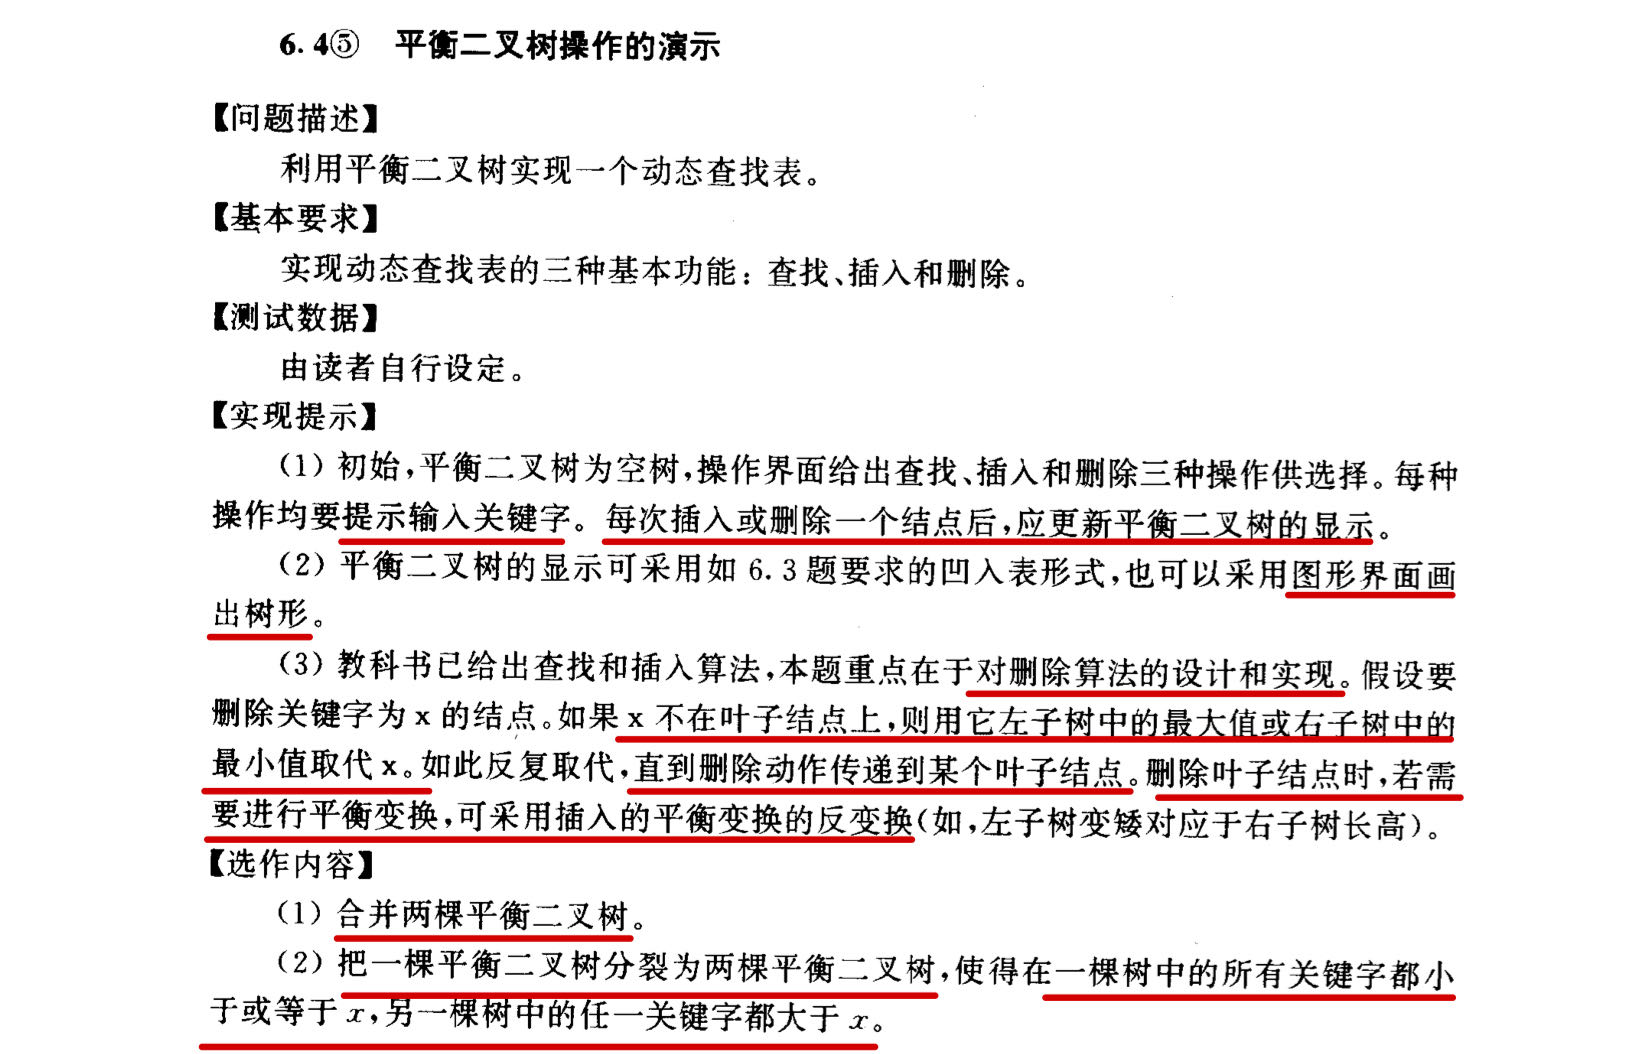
\includegraphics[width=15cm]{fig/AVLTree1.jpg}
  \caption{平衡二叉树操作的具体要求}
\end{figure}

我们需要实现的是平衡二叉树结点的插入、删除、查找,以及选作内容中的合并两棵平衡二叉树和将一棵平衡二叉树分裂为两颗平衡二叉树并满足相应的要求。下面介绍各种算法的具体实现。

\vspace{1ex}

\noindent
$\bullet$
\textbf{平衡二叉树的概念介绍}。

平衡二叉树满足如下条件:左子树和右子树深度之差的绝对值不大于1;左子树和右子树也都是平衡二叉树。特别地,空树也为平衡二叉树。

结点的平衡因子:该结点的左子树的深度减去其右子树深度。因此,平衡二叉树上每个结点的平衡因子只可能是1、0和-1。

在本实验中,我们使用的用来表示平衡二叉树的数据结构为:

% \begin{figure}[H]
%   \centering
%   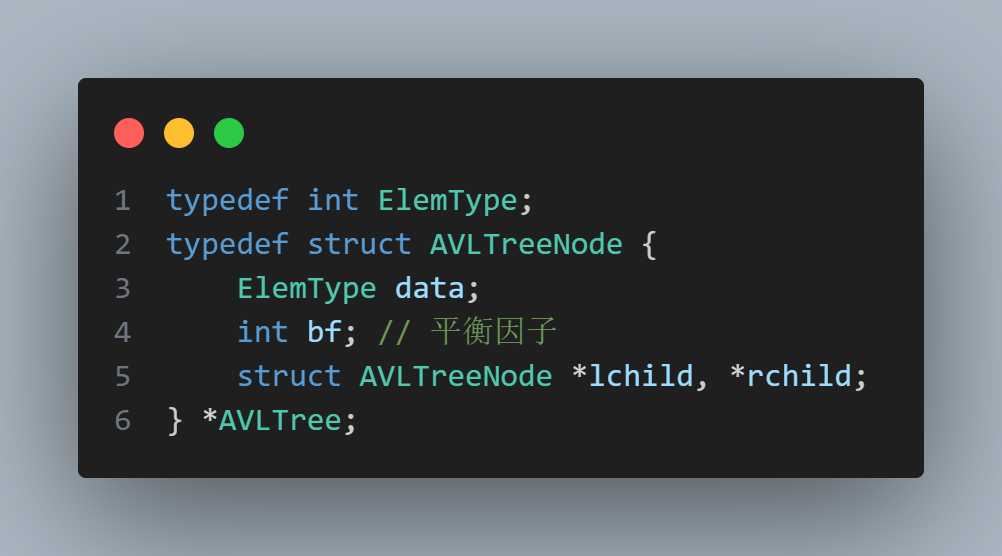
\includegraphics[width=10cm]{fig/AVLTree2.png}
%   \caption{平衡二叉树数据结构}
% \end{figure}

\begin{lstlisting}[language=C, caption={平衡二叉树数据结构}]
    typedef int ElemType;
    typedef struct AVLTreeNode {
        ElemType data;
        int bf; // 平衡因子
        struct AVLTreeNode *lchild, *rchild;
    } *AVLTree;
\end{lstlisting}

与教材上的相同。

\vspace{1ex}
\noindent
$\bullet$
\textbf{平衡化旋转}

如果在一棵平衡的二叉排序树中插入一个新结点,造成了不平衡,那么必须调整树的结构,使之平衡化。每插入/删除一个新结点时,AVL树中相关结点的平衡状态会发生改变。因此,在插入/删除一个新结点后,需要检查各结点的平衡因子,如果在某一结点发现不平衡,停止回溯。从发生不平衡的结点起,沿刚才回溯的路径取直接下两层的结点,进行平衡化旋转。

\begin{figure}[H]
  \centering
  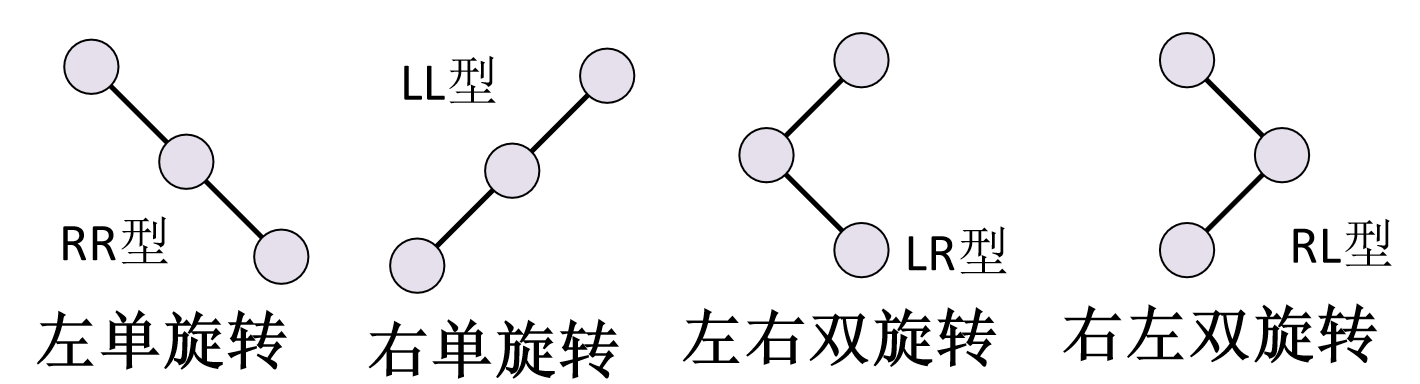
\includegraphics[width=15cm]{fig/AVLTree3.png}
  \caption{平衡化分类}
\end{figure}

如上图所示,共有四种平衡化类型,但是由于后两种类型的平衡化是由前两种类型组合而成的,因此只需要实现前两种旋转即可:

% \begin{figure}[H]
%   \centering
%   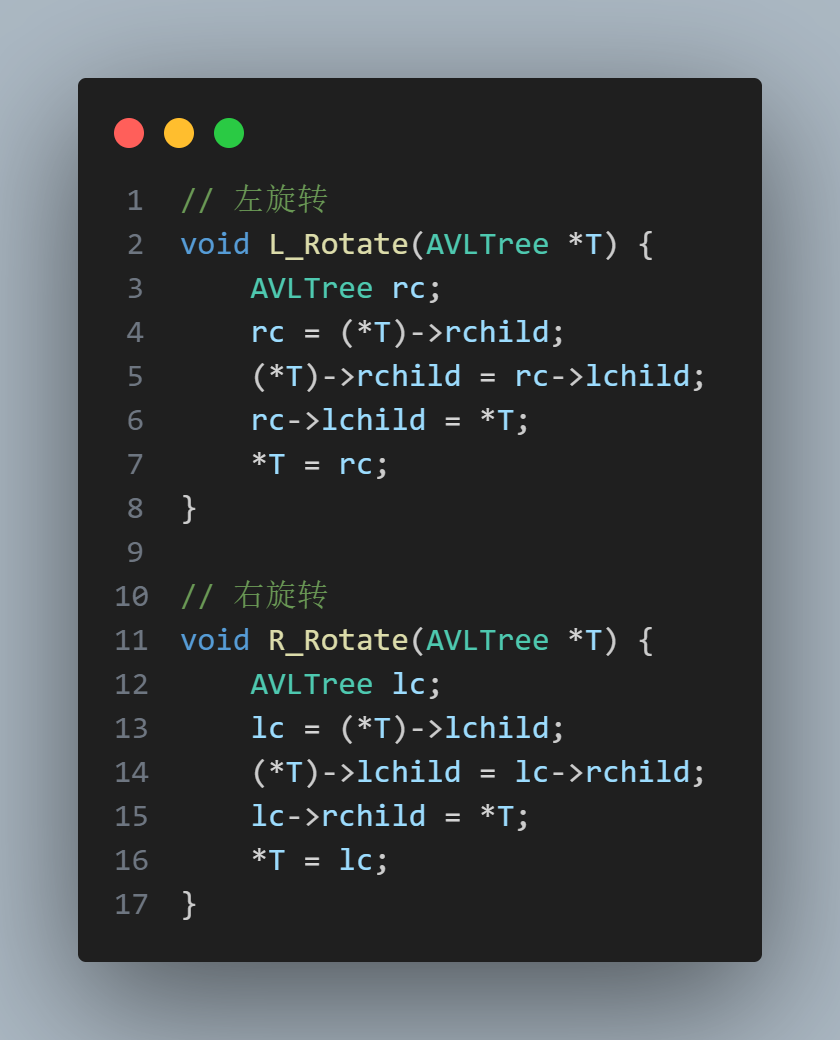
\includegraphics[width=10cm]{fig/AVLTree4.png}
%   \caption{左单旋转和右单旋转}
% \end{figure}

\begin{lstlisting}[language=C, caption={左单旋转和右单旋转}]
    // 左旋转
    void L_Rotate(AVLTree *T) {
        AVLTree rc;
        rc = (*T)->rchild;
        (*T)->rchild = rc->lchild;
        rc->lchild = *T;
        *T = rc;
    }

    // 右旋转
    void R_Rotate(AVLTree *T) {
        AVLTree lc;
        lc = (*T)->lchild;
        (*T)->lchild = lc->rchild;
        lc->rchild = *T;
        *T = lc;
    }
\end{lstlisting}

具体的操作过程和上课介绍的一样,在这里就不详细介绍了。

\vspace{1ex}

\noindent
$\bullet$
\textbf{平衡二叉树的插入}。

在向一棵本来是平衡的AVL树中插入一个新结点时,需从插入结点沿通向根的路径向上回溯,如果某个结点的平衡因子的绝对值 |bf| > 1,那么需从这个结点出发,使用平衡旋转方法进行平衡化处理。

如果一开始的平衡二叉树是空树,那么我们需要获取一定的空间,将待插入的关键字插入到根节点:

% \begin{figure}[H]
%   \centering
%   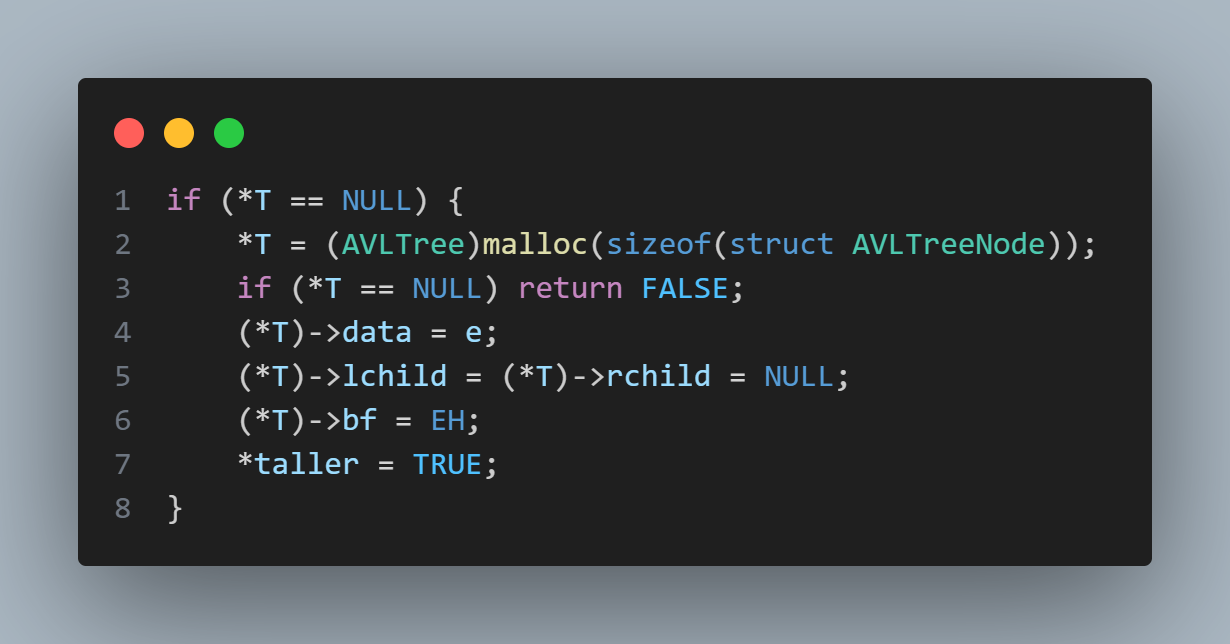
\includegraphics[width=15cm]{fig/AVLTree5.png}
%   \caption{空树的插入}
% \end{figure}

\begin{lstlisting}[language=C, caption={空树的插入}]
    if (*T == NULL) {
        *T = (AVLTree)malloc(sizeof(struct AVLTreeNode));
        if (*T == NULL) return FALSE;
        (*T)->data = e;
        (*T)->lchild = (*T)->rchild = NULL;
        (*T)->bf = EH;
        *taller = TRUE;
    }
\end{lstlisting}

如果待插入的关键字已经存在,则无法插入:

% \begin{figure}[H]
%   \centering
%   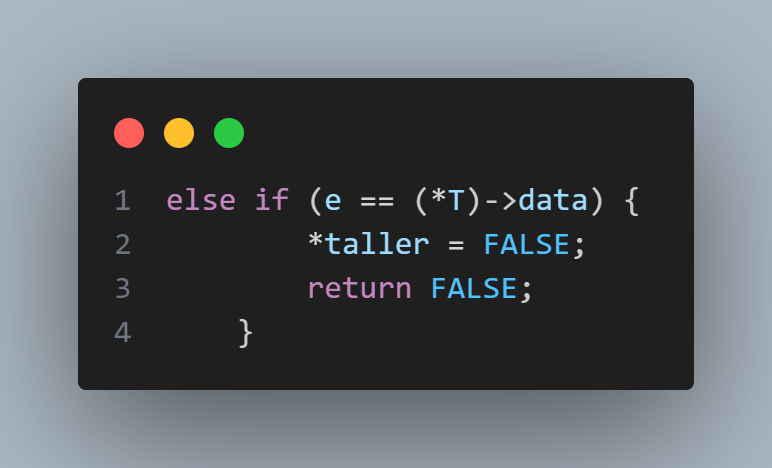
\includegraphics[width=13cm]{fig/AVLTree6.png}
%   \caption{待插入的关键字已存在}
% \end{figure}

\begin{lstlisting}[language=C, caption={待插入的关键字已存在}]
    else if (e == (*T)->data) {
        *taller = FALSE;
        return FALSE;
    }
\end{lstlisting}

排除以上特殊情况之后,设新结点p的平衡因子为0,其父结点为pr。插入新结点后,pr的平衡因子值有三种情况:

结点pr的平衡因子为0,说明刚才是在pr的较矮的子树上插入了新结点,此时不需做平衡化处理,返回主程序,子树的高度不变。

结点pr的平衡因子的绝对值|bf|\ =\ 1,说明插入前pr的平衡因子是0,插入新结点后,以pr为根的子树不需平衡化旋转。但该子树高度增加,还需从结点pr向根方向回溯,继续考查结点pr双亲(pr\ =\ Parent(pr))的平衡状态。

结点pr的平衡因子的绝对值|bf|\ =\ 2说明新结点在较高的子树上插入,造成了不平衡,需要做平衡化旋转。此时可进一步分2种情况讨论:若结点pr的bf\ =\ -2,说明右子树高,结合其右子女q的bf分别处理:若q的bf为-1,执行左单旋转;若q的bf为1,执行先右后左双旋转。若结点pr的bf\ =\ 2,说明左子树高,结合其左子女q的bf分别处理:若q的bf为1,执行右单旋转;若q的bf为-1,执行先左后右双旋转。

% \begin{figure}[H]
%   \centering
%   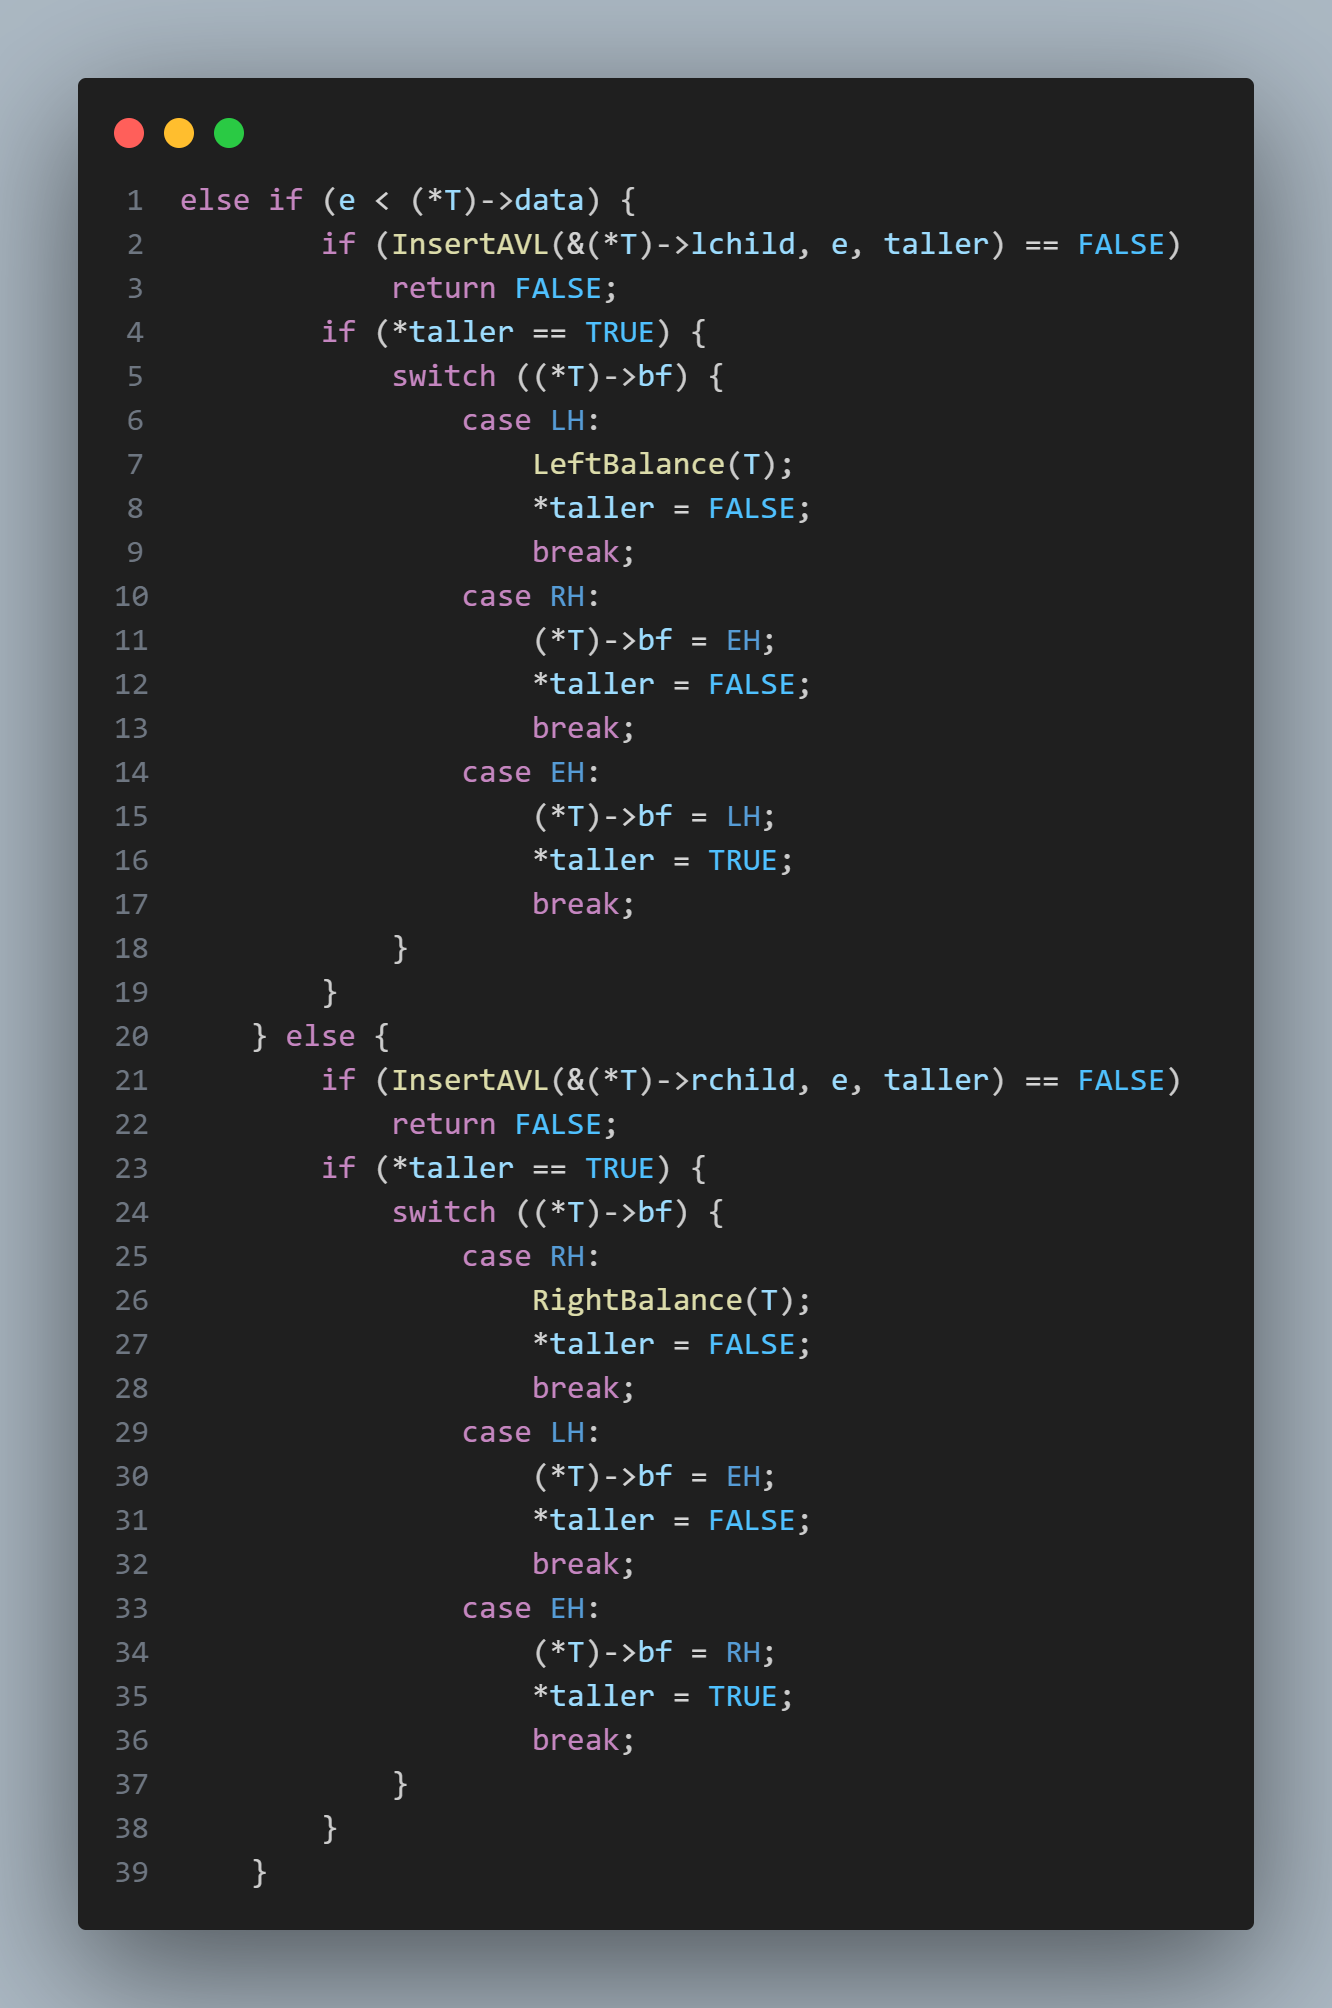
\includegraphics[width=13cm]{fig/AVLTree7.png}
%   \caption{平衡二叉树的插入}
% \end{figure}

\begin{lstlisting}[language=C, caption={平衡二叉树的插入}]
    else if (e < (*T)->data) {
        if (InsertAVL(&(*T)->lchild, e, taller) == FALSE)
            return FALSE;
        if (*taller == TRUE) {
            switch ((*T)->bf) {
                case LH:
                    LeftBalance(T);
                    *taller = FALSE;
                    break;
                case RH:
                    (*T)->bf = EH;
                    *taller = FALSE;
                    break;
                case EH:
                    (*T)->bf = LH;
                    *taller = TRUE;
                    break;
            }
        }
    } else {
        if (InsertAVL(&(*T)->rchild, e, taller) == FALSE)
            return FALSE;
        if (*taller == TRUE) {
            switch ((*T)->bf) {
                case RH:
                    RightBalance(T);
                    *taller = FALSE;
                    break;
                case LH:
                    (*T)->bf = EH;
                    *taller = FALSE;
                    break;
                case EH:
                    (*T)->bf = RH;
                    *taller = TRUE;
                    break;
            }
        }
    }
\end{lstlisting}

以上为刚刚讨论的三种情况的具体代码,可以看出主要是利用递归找到对应插入位置之后再完成相应的平衡化操作。注意这里面的LeftBalance()和RightBalance()函数则是判断平衡化的关键:

% \begin{figure}[H]
%   \centering
%   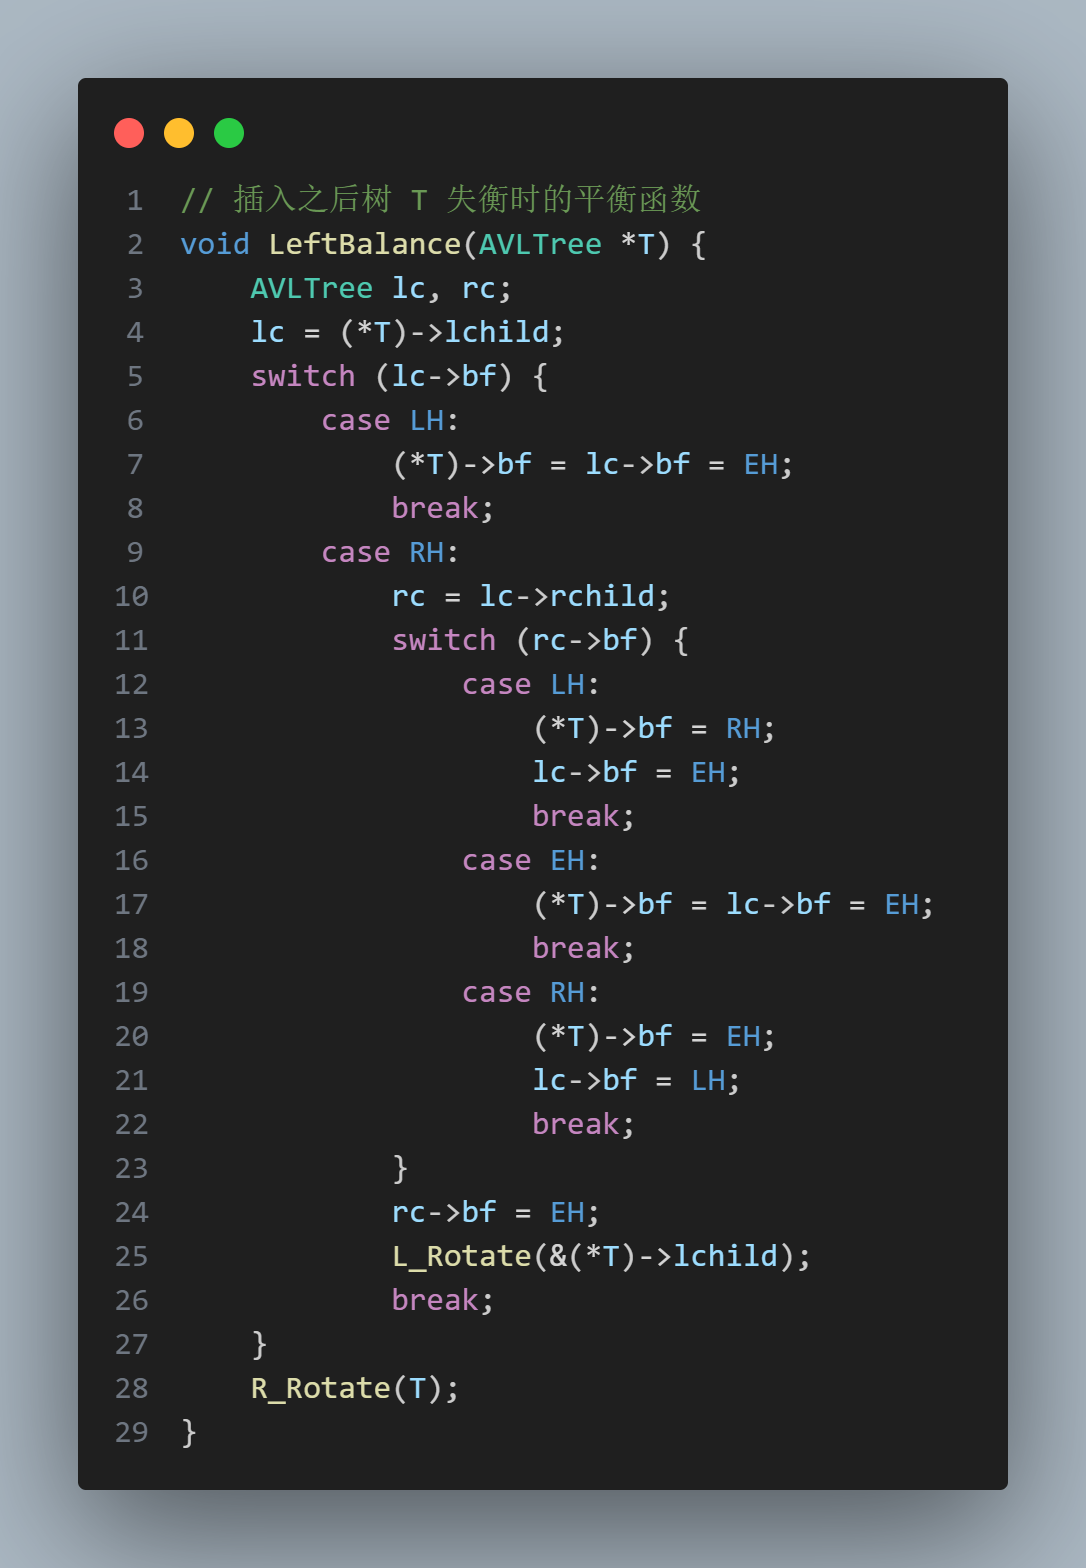
\includegraphics[width=13cm]{fig/AVLTree8.png}
%   \caption{插入后对左子树的平衡化处理}
% \end{figure}

\begin{lstlisting}[language=C, caption={插入后对左子树的平衡化处理}]
    // 插入之后树 T 失衡时的平衡函数
    void LeftBalance(AVLTree *T) {
        AVLTree lc, rc;
        lc = (*T)->lchild;
        switch (lc->bf) {
            case LH:
                (*T)->bf = lc->bf = EH;
                break;
            case RH:
                rc = lc->rchild;
                switch (rc->bf) {
                    case LH:
                        (*T)->bf = RH;
                        lc->bf = EH;
                        break;
                    case EH:
                        (*T)->bf = lc->bf = EH;
                        break;
                    case RH:
                        (*T)->bf = EH;
                        lc->bf = LH;
                        break;
                }
                rc->bf = EH;
                L_Rotate(&(*T)->lchild);
                break;
        }
        R_Rotate(T);
    }
\end{lstlisting}

% \begin{figure}[H]
%   \centering
%   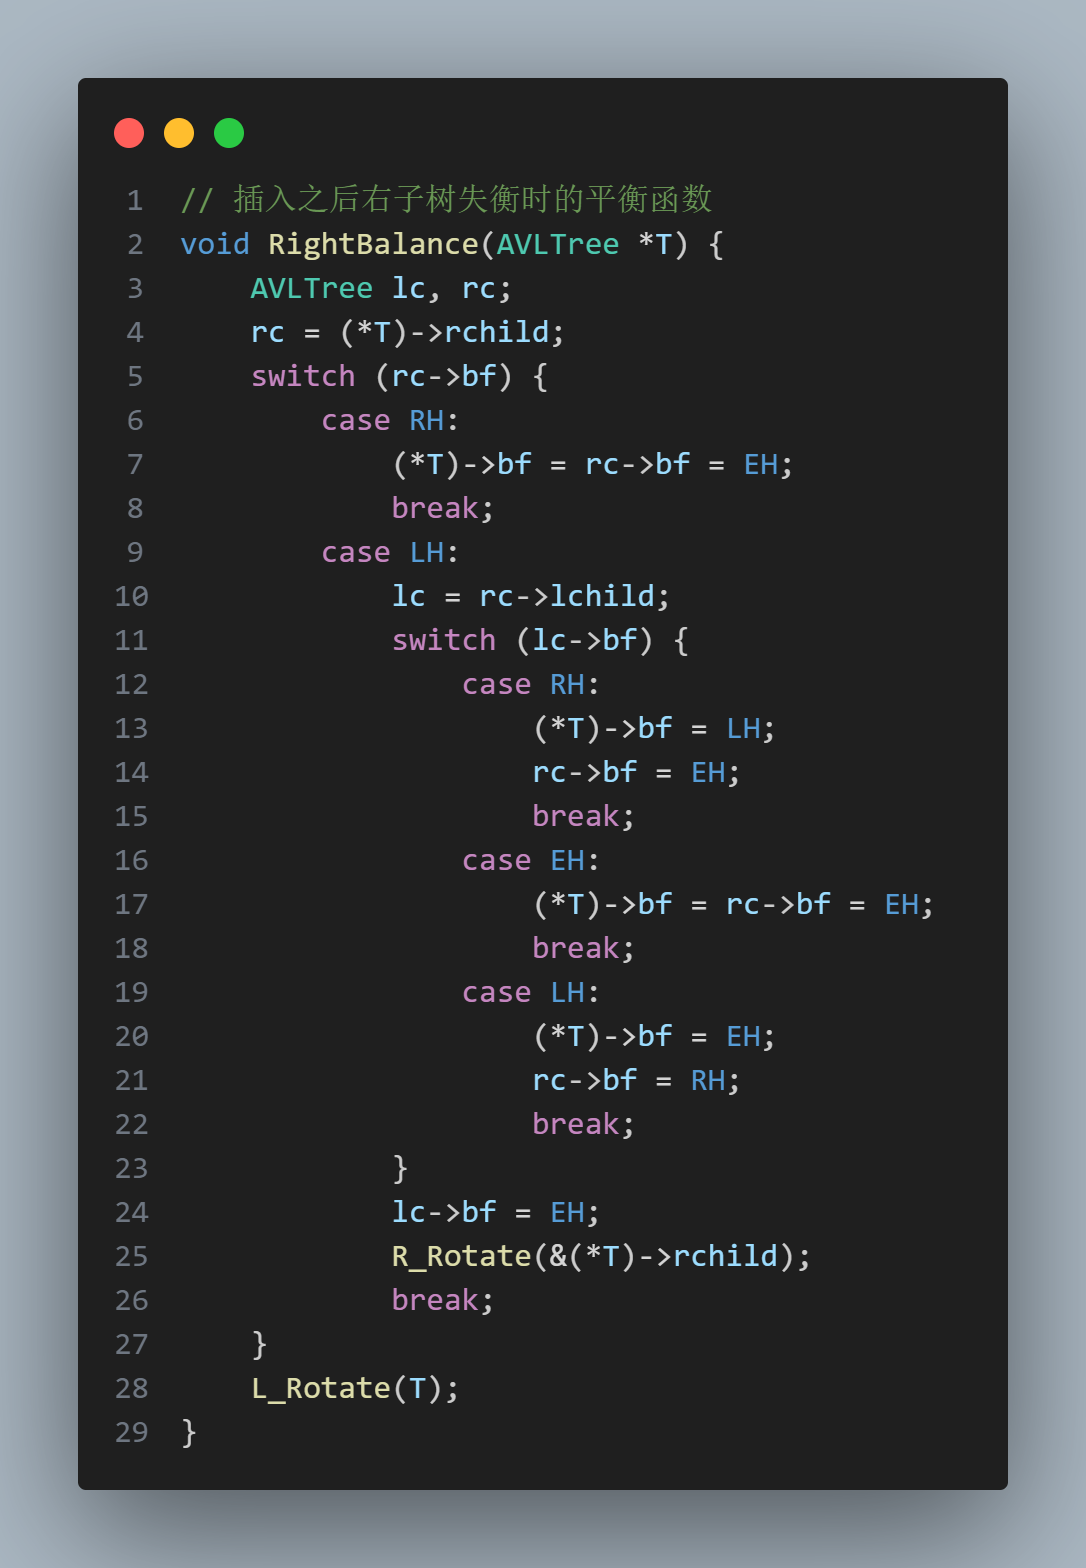
\includegraphics[width=13cm]{fig/AVLTree9.png}
%   \caption{插入后对右子树的平衡化处理}
% \end{figure}

\begin{lstlisting}[language=C, caption={插入后对右子树的平衡化处理}]
    // 插入之后右子树失衡时的平衡函数
    void RightBalance(AVLTree *T) {
        AVLTree lc, rc;
        rc = (*T)->rchild;
        switch (rc->bf) {
            case RH:
                (*T)->bf = rc->bf = EH;
                break;
            case LH:
                lc = rc->lchild;
                switch (lc->bf) {
                    case RH:
                        (*T)->bf = LH;
                        rc->bf = EH;
                        break;
                    case EH:
                        (*T)->bf = rc->bf = EH;
                        break;
                    case LH:
                        (*T)->bf = EH;
                        rc->bf = RH;
                        break;
                }
                lc->bf = EH;
                R_Rotate(&(*T)->rchild);
                break;
        }
        L_Rotate(T);
    }
\end{lstlisting}

\vspace{1ex}

\noindent
$\bullet$
\textbf{平衡二叉树的查找}。

% \begin{figure}[H]
%   \centering
%   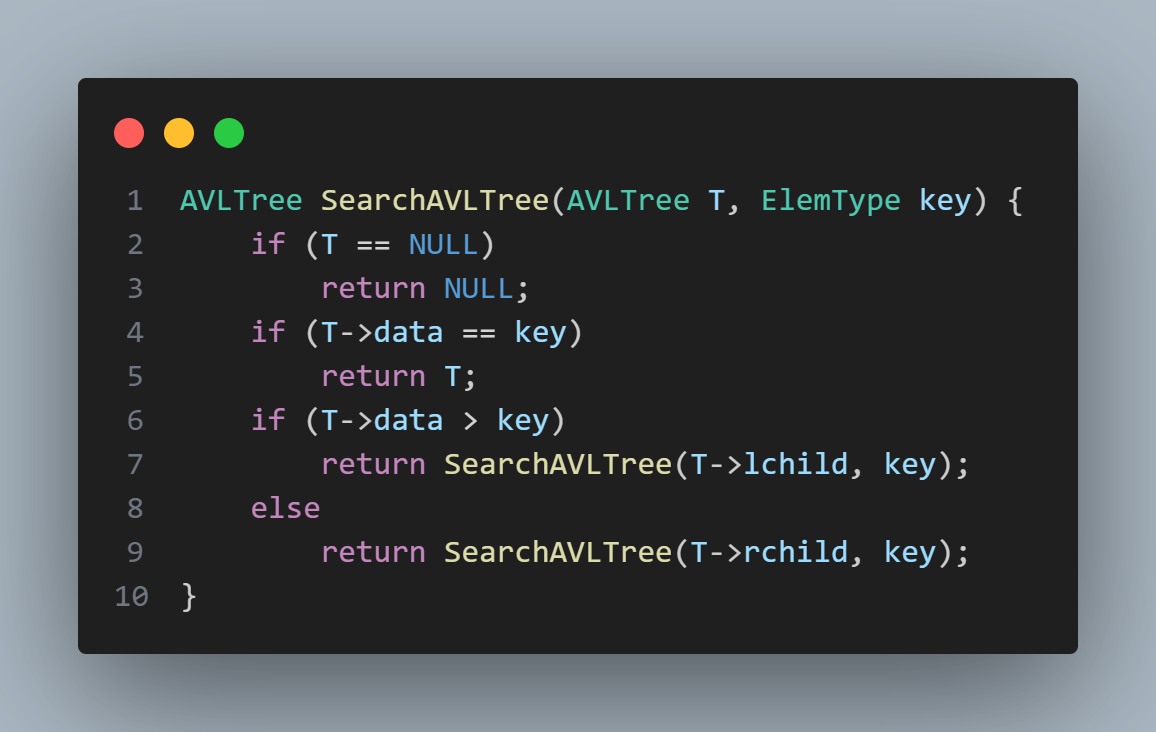
\includegraphics[width=15cm]{fig/AVLTree10.png}
%   \caption{平衡二叉树的查找}
% \end{figure}

\begin{lstlisting}[language=C, caption={平衡二叉树的查找}]
    AVLTree SearchAVLTree(AVLTree T, ElemType key) {
        if (T == NULL)
            return NULL;
        if (T->data == key)
            return T;
        if (T->data > key)
            return SearchAVLTree(T->lchild, key);
        else
            return SearchAVLTree(T->rchild, key);
    }
\end{lstlisting}

如上,平衡二叉树的查找算法就是根据带查找关键字大小和当前结点关键字大小比较,然后利用递归进行查找。

\vspace{1ex}

\noindent
$\bullet$
\textbf{平衡二叉树的删除}

如果被删结点x最多只有一个子女,可做简单地将结点x从树中删去。因为结点x最多有一个子女,可以简单地把x的双亲中原来指向x的指针改指到x的这个子女结点。如果结点x没有子女,x双亲原来指向x的指针置为NULL。再将原来以结点x为根的子树的高度减1。

如果被删结点x有两个子女,搜索x在中序次序下的直接前驱y(同样可以找直接后继),把结点y的内容传送给结点x,现在问题转移到删除结点y。把结点y当作被删结点x,因为结点y最多有一个子女,可以简单地用上述最多只有一个子女的情况进行删除,但是必须沿结点x通向根的路径反向追踪高度的变化对路径上各个结点的影响。

具体分为三种情况:

当前结点p的bf为0:如果它的左子树或右子树被缩短,则它的bf改为1或-1,同时,shorter置为False,这种情况不用旋转。

结点p的bf不为0且较高的子树被缩短:则p的bf改为0,同时shorter置为True,这种情况也不用旋转。

结点p的bf不为0,且较矮的子树又被缩短,则在结点p发生不平衡,需要进行平衡化旋转来恢复平衡:如果q(较高的子树)的bf为0,执行一个单旋转来恢复结点p的平衡,置shorter为False,无需检查上层结点的平衡因子;如果q bf与p的bf相同,则执行一个单旋转来恢复平衡,结点p和q的bf均改为0,同时置shorter为True,还要继续检查上层结点的平衡因子;如果p与q的bf相反,则执行一个双旋转来恢复平衡。先围绕q转再围绕p转,新根结点的bf置为0,其他结点的bf相应处理,同时置shorter为True。

% \begin{figure}[H]
%   \centering
%   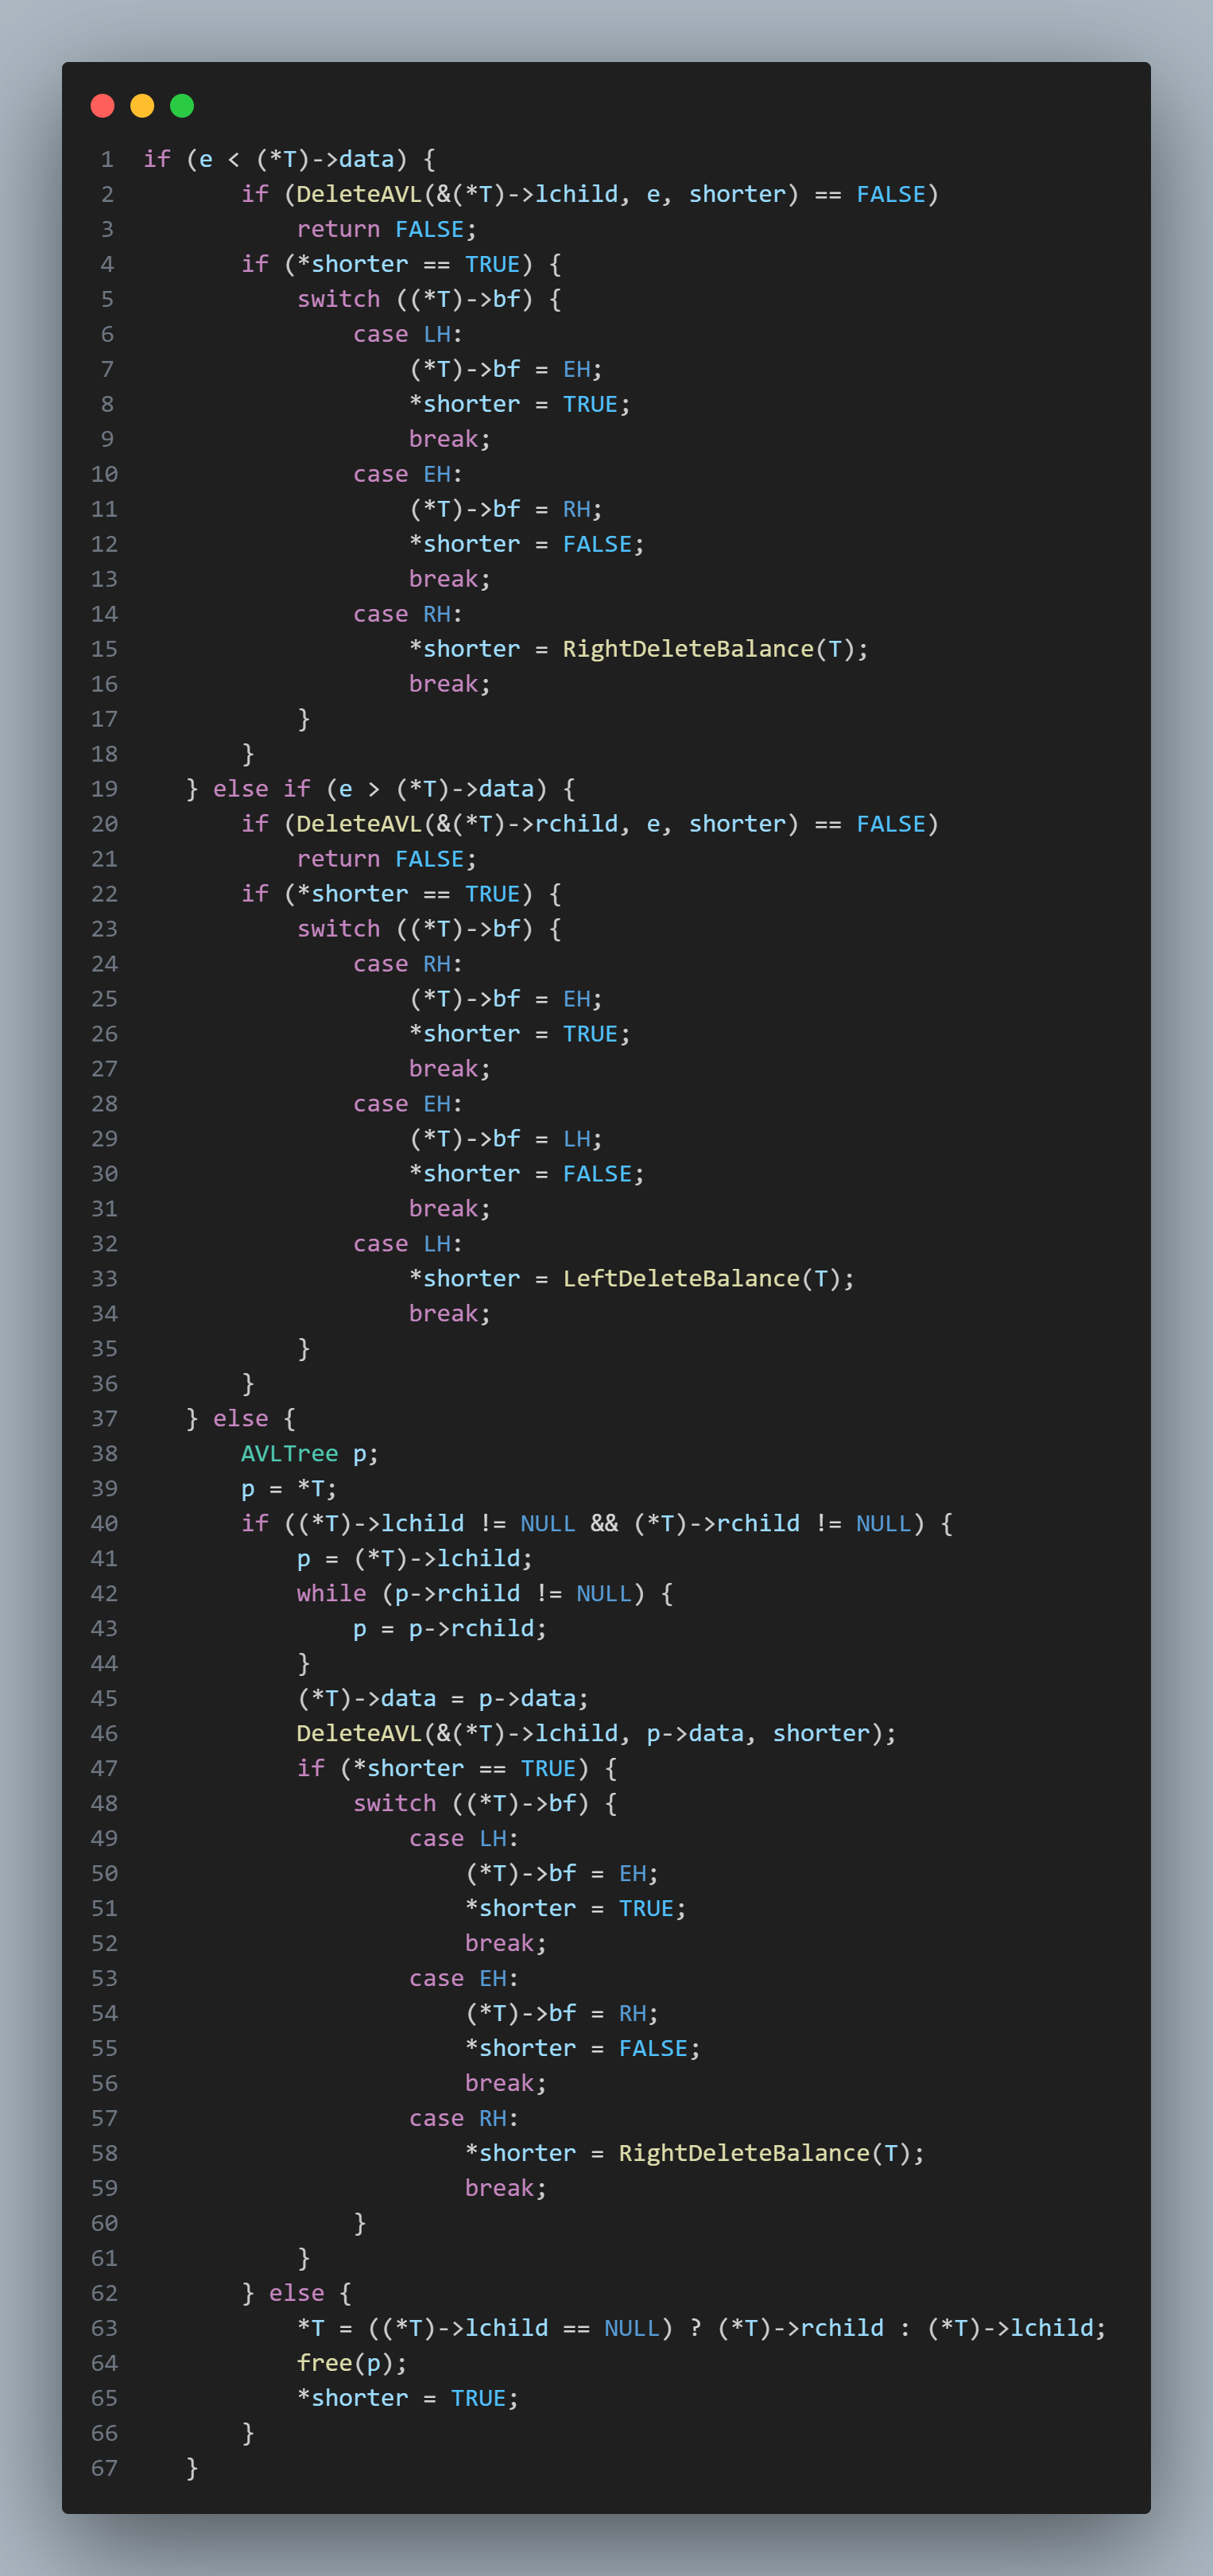
\includegraphics[width=10cm]{fig/AVLTree11.png}
%   \caption{平衡二叉树的删除}
% \end{figure}

\begin{lstlisting}[language=C, caption={平衡二叉树的删除}]
    if (e < (*T)->data) {
        if (DeleteAVL(&(*T)->lchild, e, shorter) == FALSE)
            return FALSE;
        if (*shorter == TRUE) {
            switch ((*T)->bf) {
                case LH:
                    (*T)->bf = EH;
                    *shorter = TRUE;
                    break;
                case EH:
                    (*T)->bf = RH;
                    *shorter = FALSE;
                    break;
                case RH:
                    *shorter = RightDeleteBalance(T);
                    break;
            }
        }
    } else if (e > (*T)->data) {
        if (DeleteAVL(&(*T)->rchild, e, shorter) == FALSE)
            return FALSE;
        if (*shorter == TRUE) {
            switch ((*T)->bf) {
                case RH:
                    (*T)->bf = EH;
                    *shorter = TRUE;
                    break;
                case EH:
                    (*T)->bf = LH;
                    *shorter = FALSE;
                    break;
                case LH:
                    *shorter = LeftDeleteBalance(T);
                    break;
            }
        }
    } else {
        AVLTree p;
        p = *T;
        if ((*T)->lchild != NULL && (*T)->rchild != NULL) {
            p = (*T)->lchild;
            while (p->rchild != NULL) {
                p = p->rchild;
            }
            (*T)->data = p->data;
            DeleteAVL(&(*T)->lchild, p->data, shorter);
            if (*shorter == TRUE) {
                switch ((*T)->bf) {
                    case LH:
                        (*T)->bf = EH;
                        *shorter = TRUE;
                        break;
                    case EH:
                        (*T)->bf = RH;
                        *shorter = FALSE;
                        break;
                    case RH:
                        *shorter = RightDeleteBalance(T);
                        break;
                }
            }
        } else {
            *T = ((*T)->lchild == NULL) ? (*T)->rchild : (*T)->lchild;
            free(p);
            *shorter = TRUE;
        }
    }
\end{lstlisting}

以上为刚刚讨论的三种情况的具体代码,可以看出主要是利用递归找到应该删除的结点对应位置之后再完成相应的平衡化操作。注意这里面的LeftDeleteBalance()和RightDeleteBalance()函数则是判断平衡化的关键:

% \begin{figure}[H]
%   \centering
%   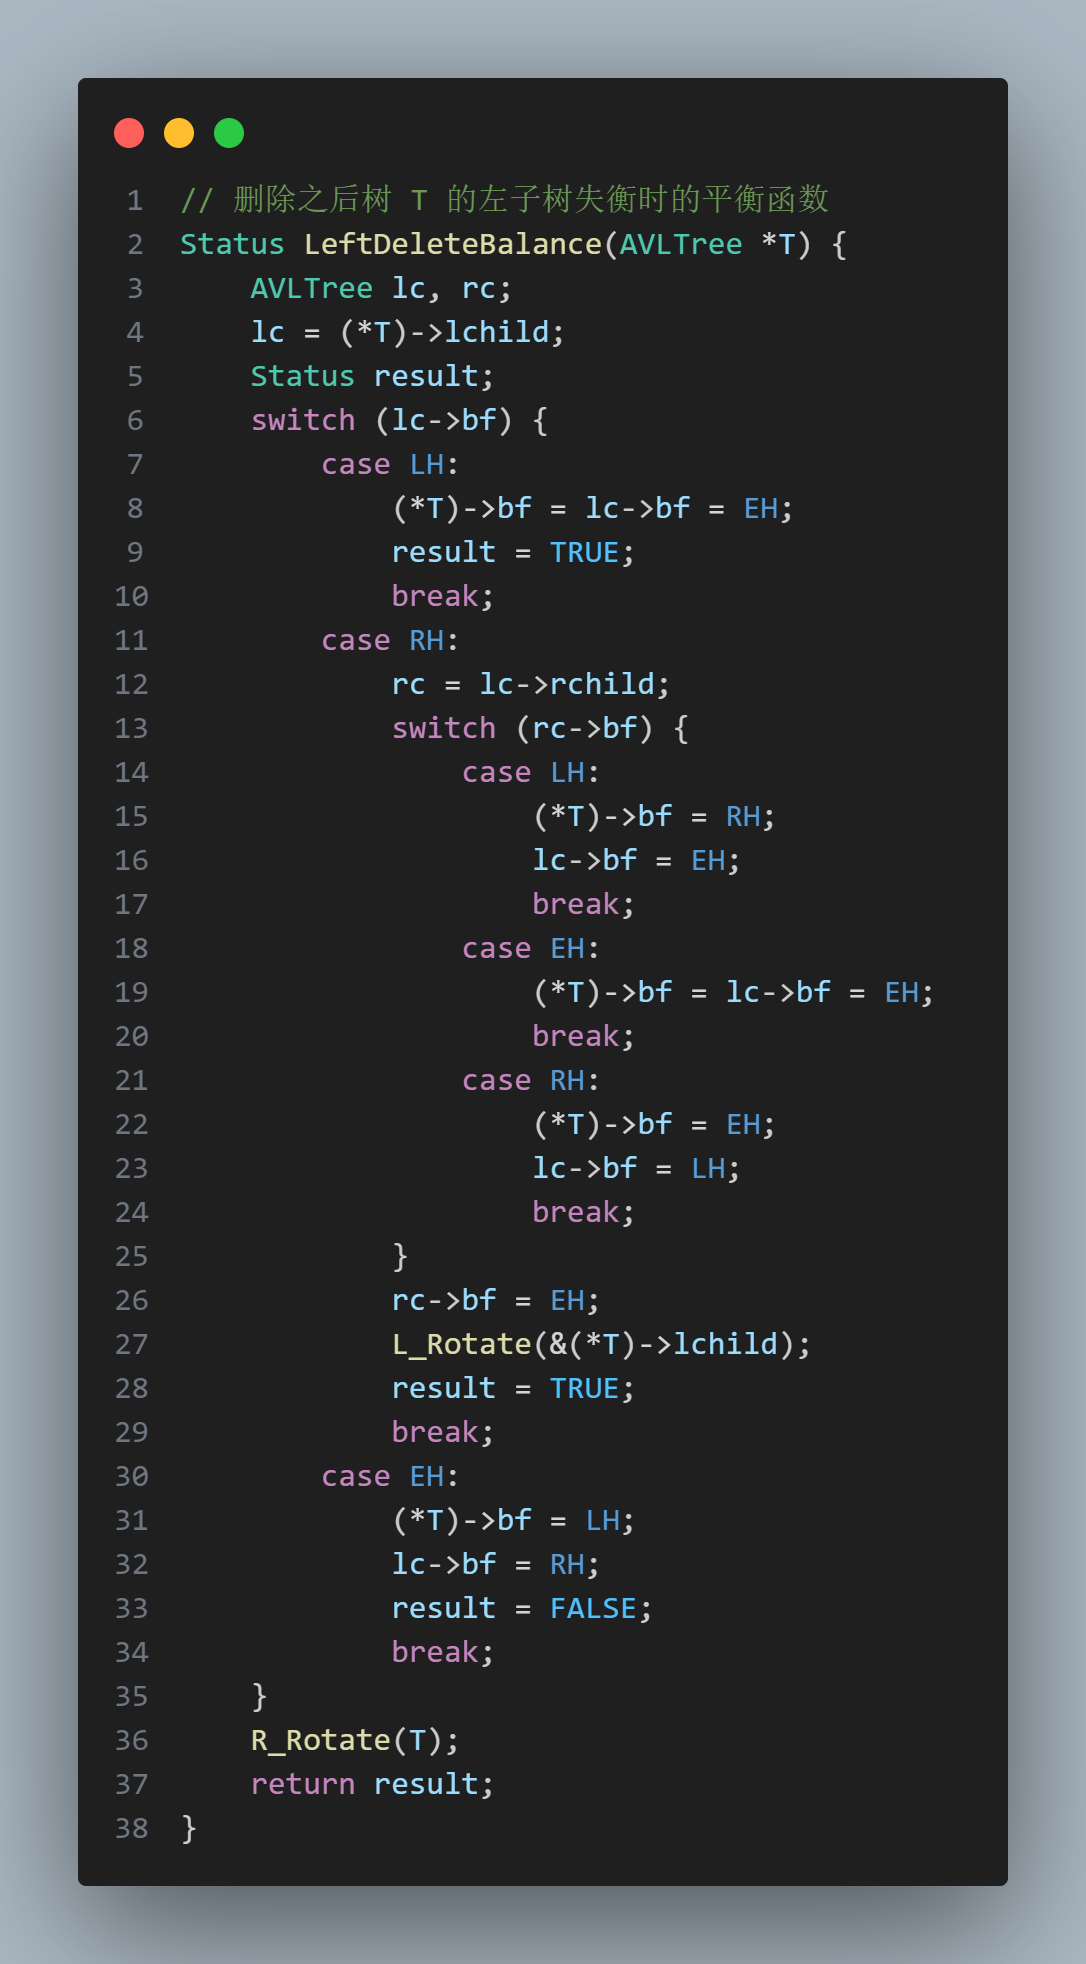
\includegraphics[width=13cm]{fig/AVLTree12.png}
%   \caption{删除后对左子树的平衡化处理}
% \end{figure}

\begin{lstlisting}[language=C, caption={删除后对左子树的平衡化处理}]
    // 删除之后树 T 的左子树失衡时的平衡函数
    Status LeftDeleteBalance(AVLTree *T) {
        AVLTree lc, rc;
        lc = (*T)->lchild;
        Status result;
        switch (lc->bf) {
            case LH:
                (*T)->bf = lc->bf = EH;
                result = TRUE;
                break;
            case RH:
                rc = lc->rchild;
                switch (rc->bf) {
                    case LH:
                        (*T)->bf = RH;
                        lc->bf = EH;
                        break;
                    case EH:
                        (*T)->bf = lc->bf = EH;
                        break;
                    case RH:
                        (*T)->bf = EH;
                        lc->bf = LH;
                        break;
                }
                rc->bf = EH;
                L_Rotate(&(*T)->lchild);
                result = TRUE;
                break;
            case EH:
                (*T)->bf = LH;
                lc->bf = RH;
                result = FALSE;
                break;
        }
        R_Rotate(T);
        return result;
    }
\end{lstlisting}

% \begin{figure}[H]
%   \centering
%   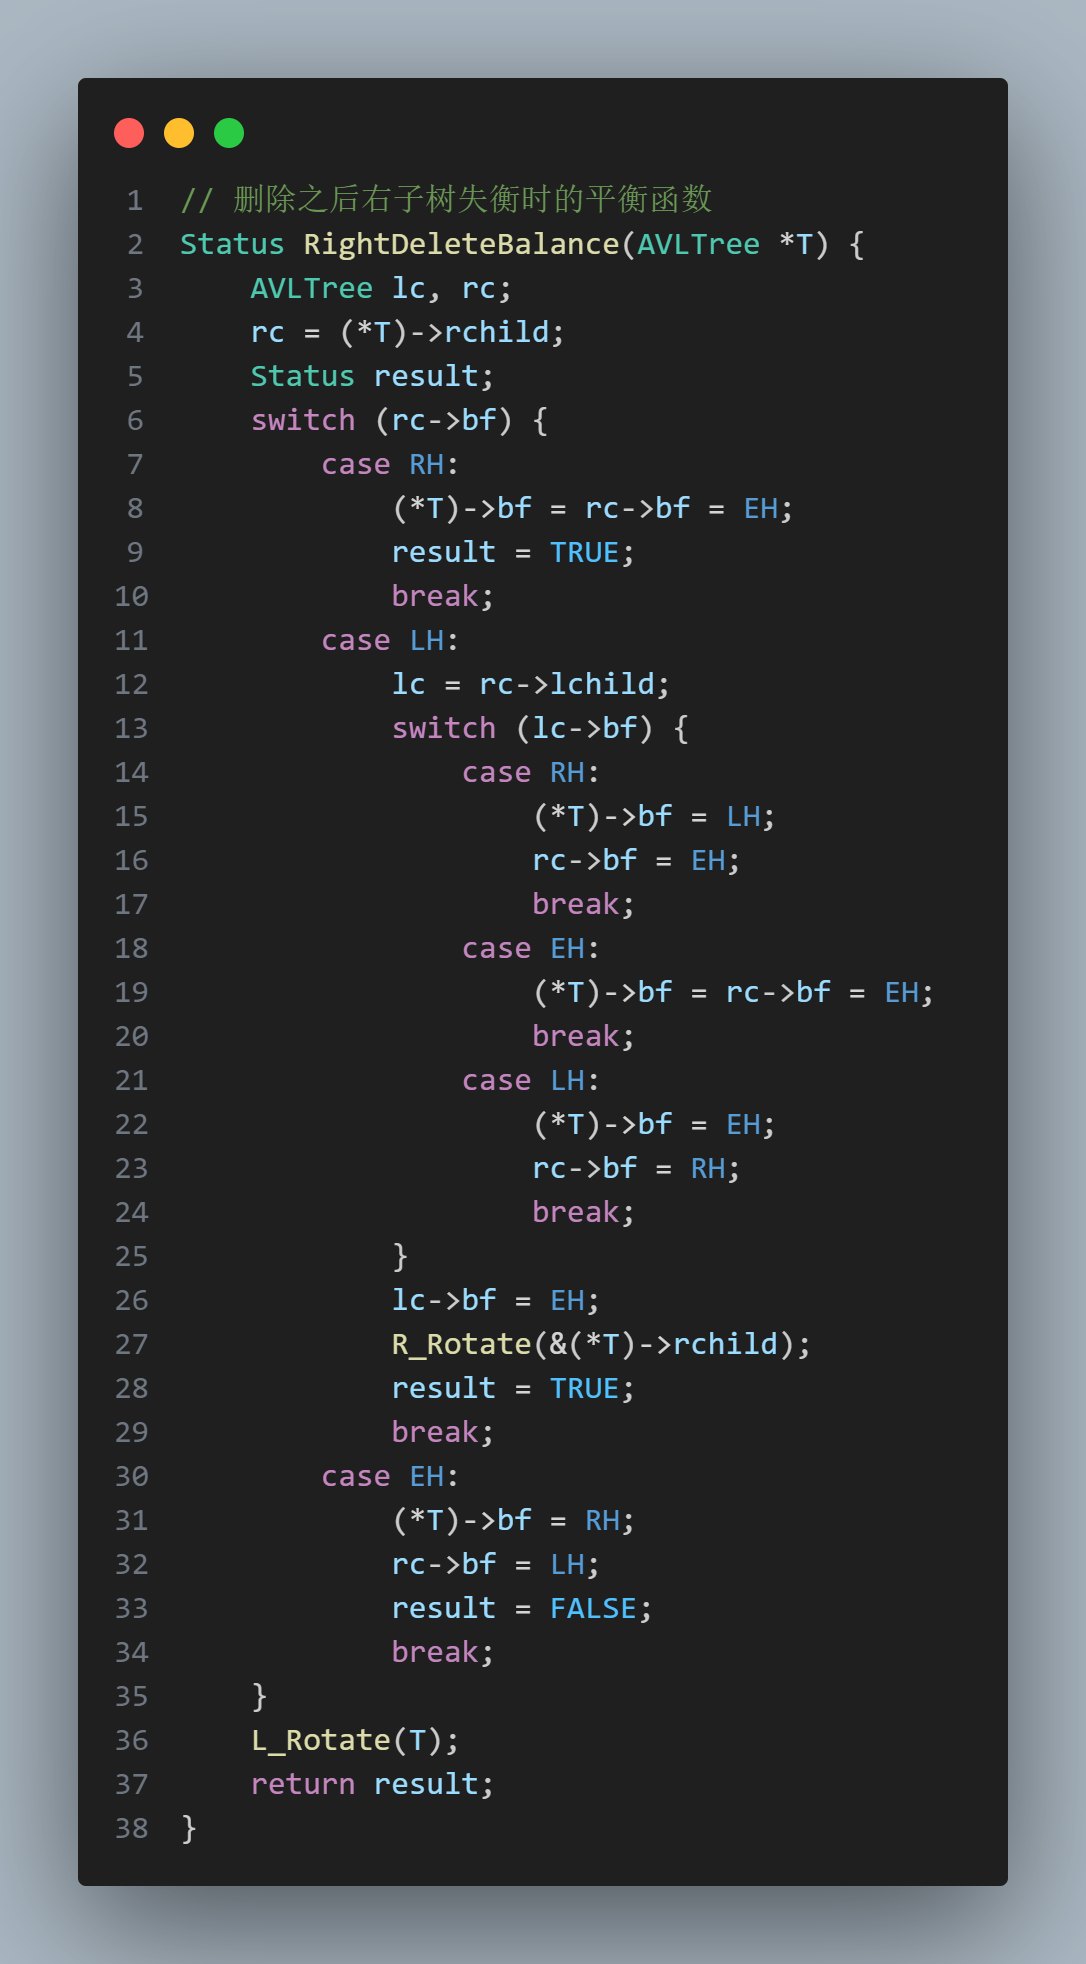
\includegraphics[width=13cm]{fig/AVLTree13.png}
%   \caption{删除后对右子树的平衡化处理}
% \end{figure}

\begin{lstlisting}[language=C, caption={删除后对右子树的平衡化处理}]
    // 删除之后右子树失衡时的平衡函数
    Status RightDeleteBalance(AVLTree *T) {
        AVLTree lc, rc;
        rc = (*T)->rchild;
        Status result;
        switch (rc->bf) {
            case RH:
                (*T)->bf = rc->bf = EH;
                result = TRUE;
                break;
            case LH:
                lc = rc->lchild;
                switch (lc->bf) {
                    case RH:
                        (*T)->bf = LH;
                        rc->bf = EH;
                        break;
                    case EH:
                        (*T)->bf = rc->bf = EH;
                        break;
                    case LH:
                        (*T)->bf = EH;
                        rc->bf = RH;
                        break;
                }
                lc->bf = EH;
                R_Rotate(&(*T)->rchild);
                result = TRUE;
                break;
            case EH:
                (*T)->bf = RH;
                rc->bf = LH;
                result = FALSE;
                break;
        }
        L_Rotate(T);
        return result;
    }
\end{lstlisting}

\vspace{1ex}

\noindent
$\bullet$
\textbf{平衡二叉树的合并}

关于二叉树的合并,常规思路是将一棵结点数较小的平衡二叉树中的结点一个一个的插入到结点数较大的平衡二叉树中,但这样就没有利用到两棵树都是平衡二叉树的有利条件,从而导致时间、空间复杂度的提高。因此,我们组想到的方法是,先用中序遍历将两棵二叉树存储到数组中,再利用有序数组的排序合并成一个有序数组,然后再根据该有序数组的特性,每次选择中间的关键字进行插入,然后进行递归,从而优化了时间和空间复杂度。

% \begin{figure}[H]
%   \centering
%   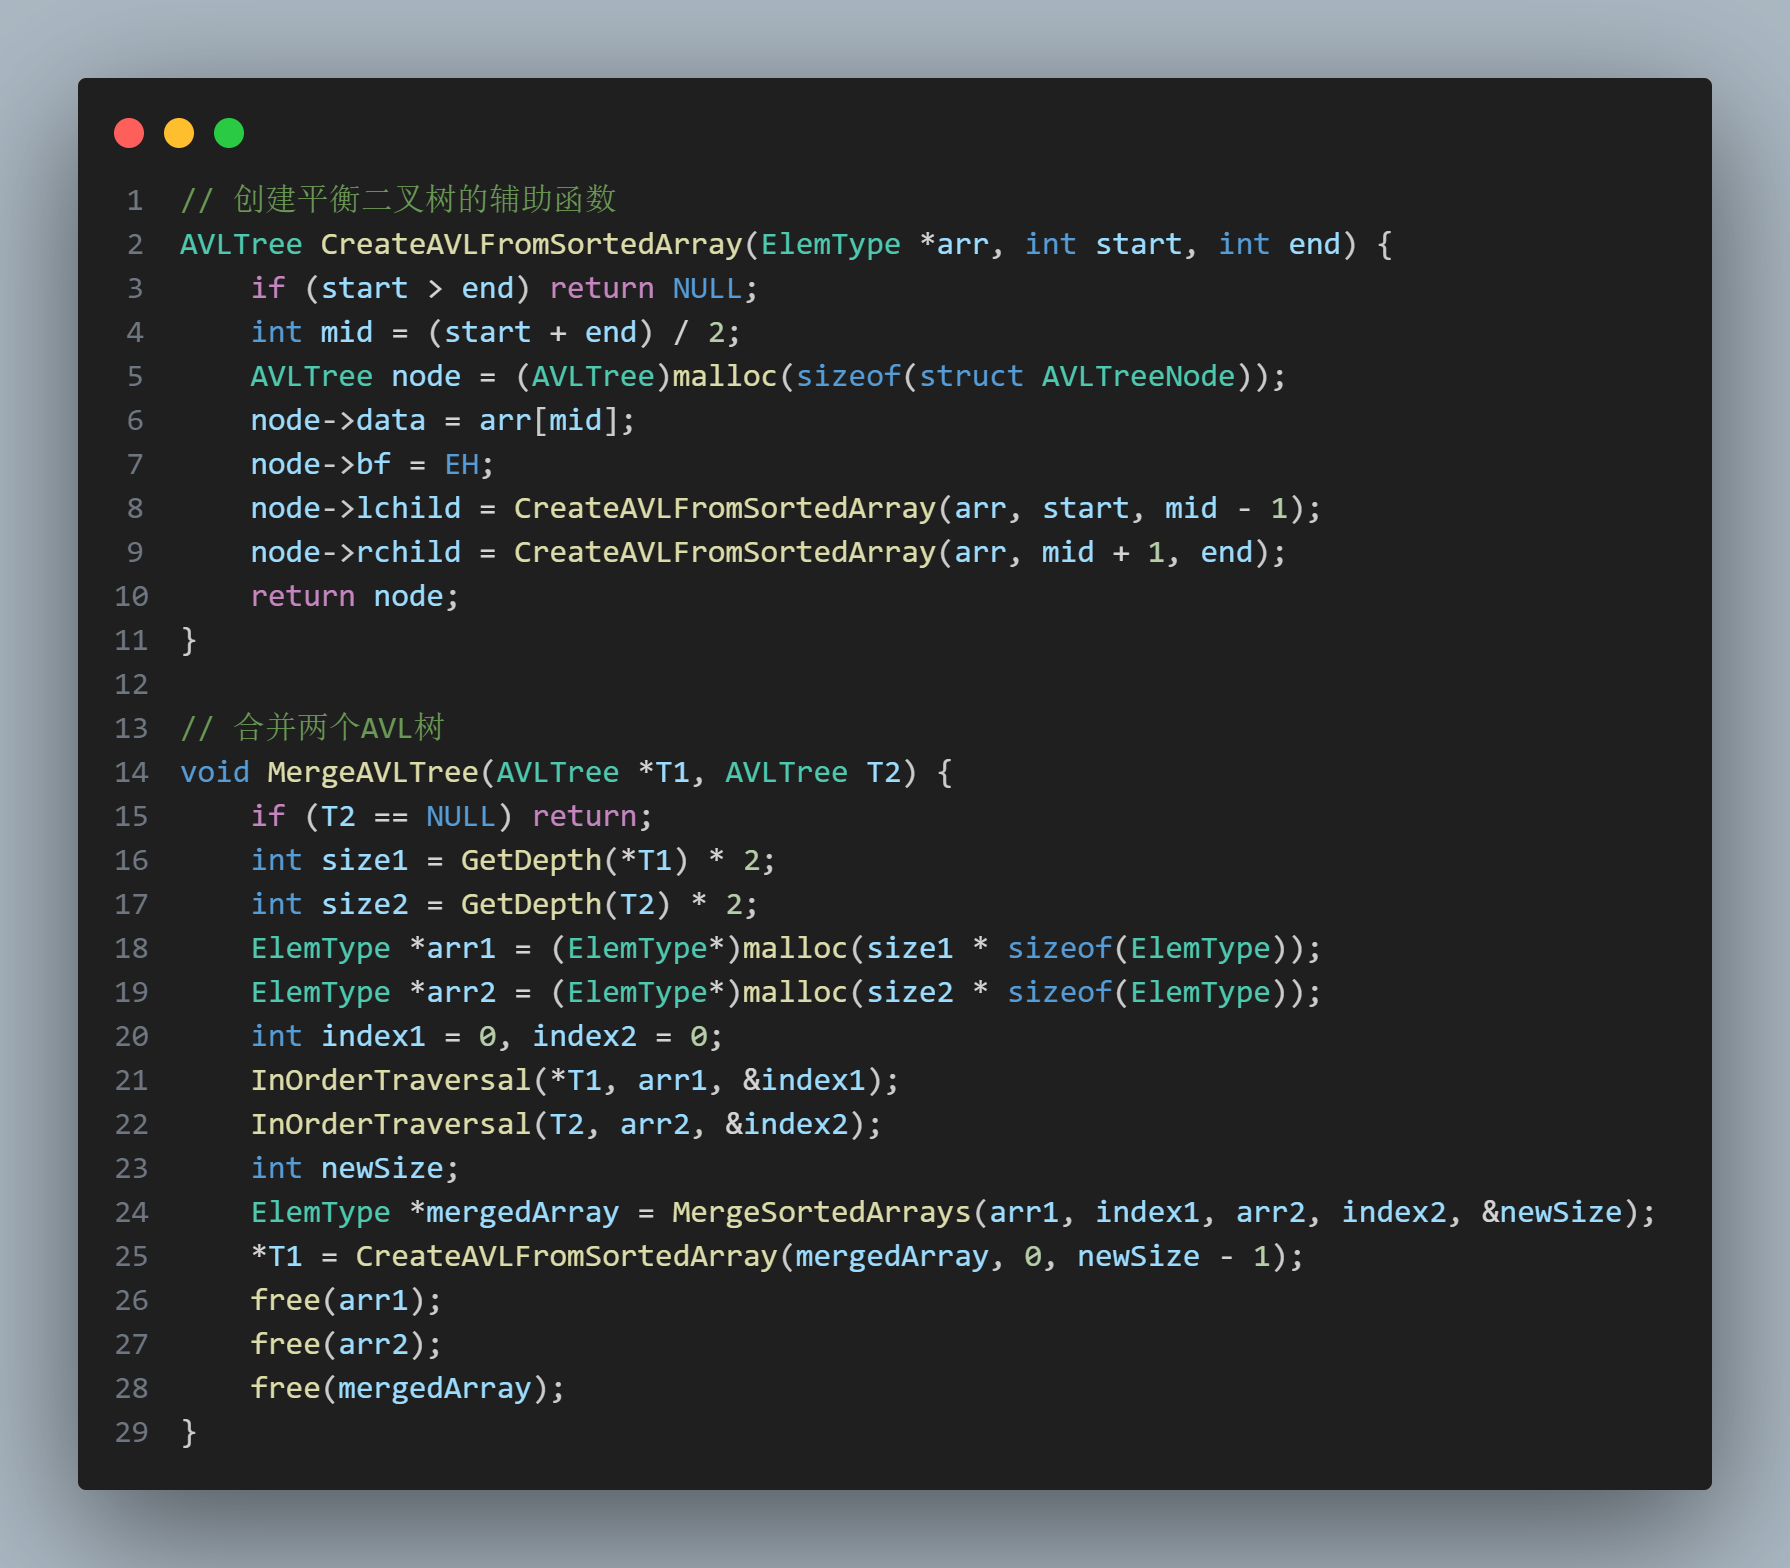
\includegraphics[width=15cm]{fig/AVLTree14.png}
%   \caption{平衡二叉树的合并}
% \end{figure}

\begin{lstlisting}[language=C, caption={平衡二叉树的合并}]
    // 创建平衡二叉树的辅助函数
    AVLTree CreateAVLFromSortedArray(ElemType *arr, int start, int end) {
        if (start > end) return NULL;
        int mid = (start + end) / 2;
        AVLTree node = (AVLTree)malloc(sizeof(struct AVLTreeNode));
        node->data = arr[mid];
        node->bf = EH;
        node->lchild = CreateAVLFromSortedArray(arr, start, mid - 1);
        node->rchild = CreateAVLFromSortedArray(arr, mid + 1, end);
        return node;
    }

    // 合并两个AVL树
    void MergeAVLTree(AVLTree *T1, AVLTree T2) {
        if (T2 == NULL) return;
        int size1 = GetDepth(*T1) * 2;
        int size2 = GetDepth(T2) * 2;
        ElemType *arr1 = (ElemType*)malloc(size1 * sizeof(ElemType));
        ElemType *arr2 = (ElemType*)malloc(size2 * sizeof(ElemType));
        int index1 = 0, index2 = 0;
        InOrderTraversal(*T1, arr1, &index1);
        InOrderTraversal(T2, arr2, &index2);
        int newSize;
        ElemType *mergedArray = MergeSortedArrays(arr1, index1, arr2, index2, &newSize);
        *T1 = CreateAVLFromSortedArray(mergedArray, 0, newSize - 1);
        free(arr1);
        free(arr2);
        free(mergedArray);
    }
\end{lstlisting}

上图为两个平衡二叉树合并的关键函数,CreateAVLFromSortedArray()函数的主要作用是根据得到的有序数组通过求出中间关键字进行插入。MergeAVLTree()则是合并的主函数。

\vspace{1ex}

\noindent
$\bullet$
\textbf{平衡二叉树的分裂}

平衡二叉树的分裂也是如此,常规思路是遍历整个二叉树,与标准比较,小于等于标准的插入一棵新的平衡二叉树,大于标准的插入另一棵平衡二叉树,但这样也没有充分利用平衡二叉树的有利条件,因此为了降低时间和空间复杂度,我们采用中序遍历平衡二叉树得到相对应的有序数组,然后将数组分成两个有序数组,按照上述合并二叉树中的方式构造两棵新的平衡二叉树。

% \begin{figure}[H]
%   \centering
%   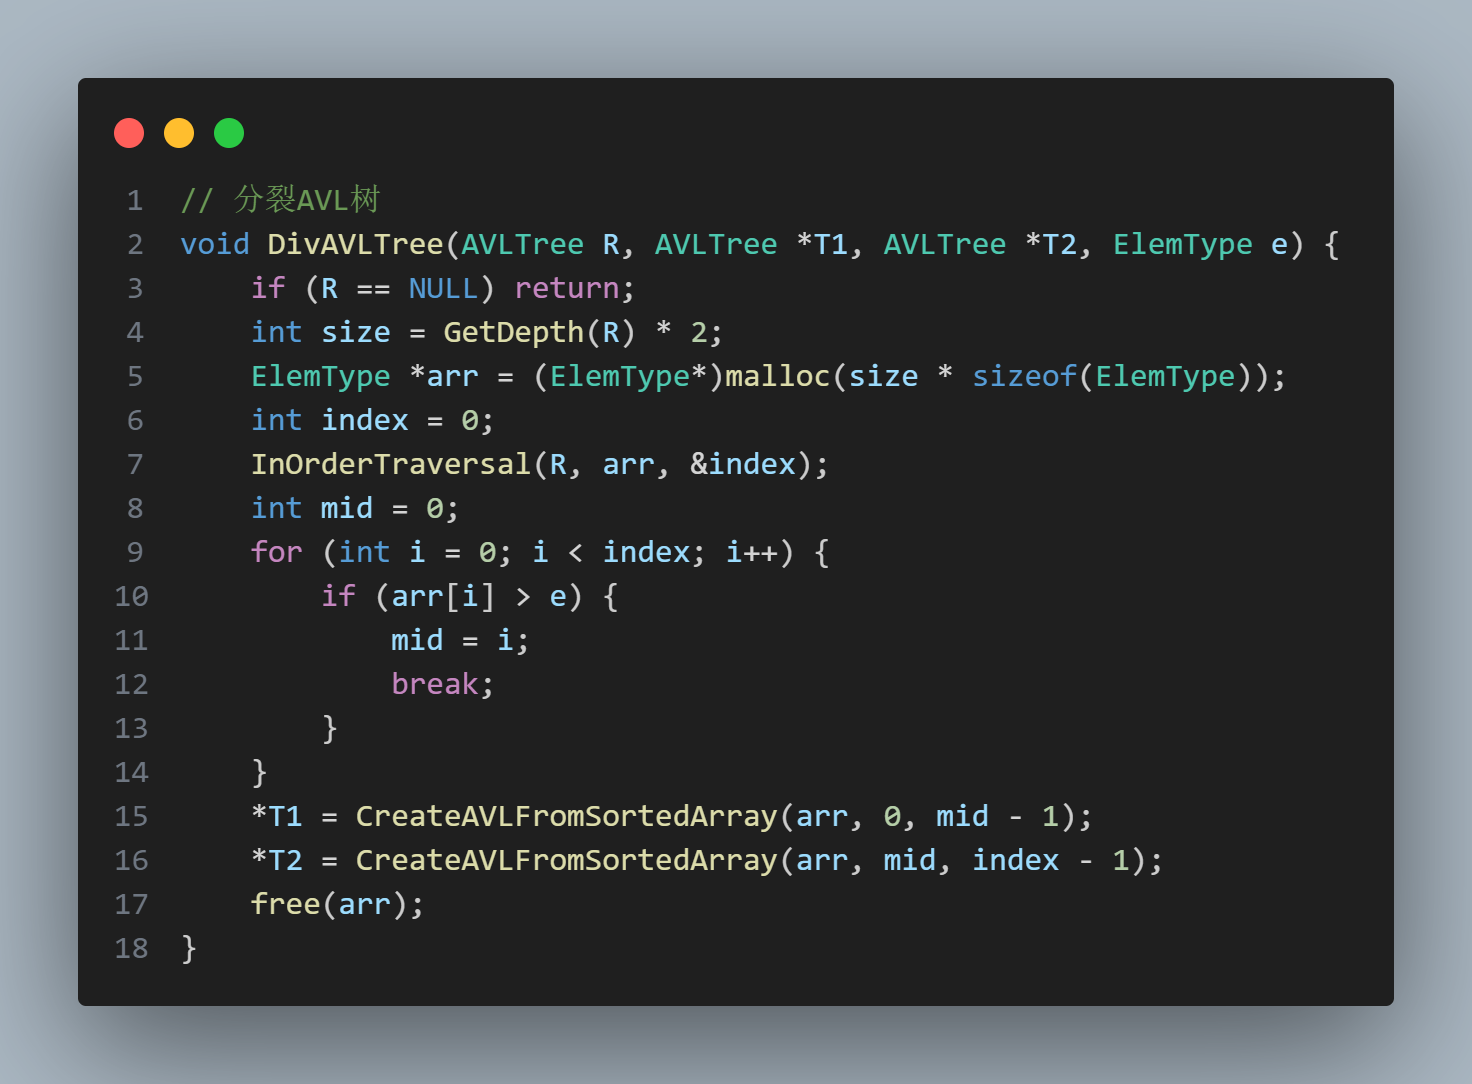
\includegraphics[width=15cm]{fig/AVLTree15.png}
%   \caption{平衡二叉树的分裂}
% \end{figure}

\begin{lstlisting}[language=C, caption={平衡二叉树的分裂}]
    // 分裂AVL树
    void DivAVLTree(AVLTree R, AVLTree *T1, AVLTree *T2, ElemType e) {
        if (R == NULL) return;
        int size = GetDepth(R) * 2;
        ElemType *arr = (ElemType*)malloc(size * sizeof(ElemType));
        int index = 0;
        InOrderTraversal(R, arr, &index);
        int mid = 0;
        for (int i = 0; i < index; i++) {
            if (arr[i] > e) {
                mid = i;
                break;
            }
        }
        *T1 = CreateAVLFromSortedArray(arr, 0, mid - 1);
        *T2 = CreateAVLFromSortedArray(arr, mid, index - 1);
        free(arr);
    }
\end{lstlisting}

\subsection{时空性能分析}

\noindent
$\bullet$
\textbf{插入操作的时空复杂度}。

插入操作在AVL树中涉及查找正确的插入位置和可能的旋转操作来保持树的平衡。

查找位置: 由于AVL树是平衡二叉搜索树,其查找时间复杂度为O(log n)。

旋转操作: 每次旋转的时间复杂度为O(1)。

因此,插入操作的总时间复杂度为O(log n)。

插入操作过程中没有额外的空间消耗,空间复杂度主要来源于递归调用的栈空间。递归调用的深度为O(log n),所以空间复杂度为O(log n)。

\vspace{1ex}

\noindent
$\bullet$
\textbf{查找操作的时空复杂度}。

因为AVL树是平衡的,每次比较都可以将查找空间减半,因此查找操作在AVL树中的时间复杂度为O(log n)。

查找操作过程中没有额外的空间消耗,空间复杂度主要来源于递归调用的栈空间。递归调用的深度为O(log n),所以空间复杂度为O(log n)。

\vspace{1ex}

\noindent
$\bullet$
\textbf{删除操作的时空复杂度}

删除操作在AVL树中涉及查找节点、删除节点和可能的旋转操作来保持树的平衡。

查找节点: 时间复杂度为O(log n)。

删除节点: 如果要删除的节点有两个子节点,需要找到前驱或后继节点,操作的时间复杂度为O(log n)。

旋转操作: 每次旋转的时间复杂度为O(1)。

因此,删除操作的总时间复杂度为O(log n)。

删除操作过程中没有额外的空间消耗,空间复杂度主要来源于递归调用的栈空间。递归调用的深度为O(log n),所以空间复杂度为O(log n)。

\vspace{1ex}

\noindent
$\bullet$
\textbf{合并操作的时空复杂度}

合并操作包括以下步骤:

中序遍历两棵树: 每棵树的中序遍历时间复杂度为O(n1)和O(n2),其中n1和n2分别是两棵树的节点数。

合并两个有序数组: 时间复杂度为O(n1 + n2)。

从合并后的有序数组创建新的AVL树: 时间复杂度为O(n1 + n2)。

总时间复杂度为O(n1 + n2)。

需要额外的空间存储中序遍历的结果和合并后的有序数组,空间复杂度为O(n1 + n2)。

\vspace{1ex}

\noindent
$\bullet$
\textbf{合并操作的时空复杂度}

分裂操作包括以下步骤:

中序遍历树: 时间复杂度为O(n),其中n是树的节点数。

分割有序数组: 时间复杂度为O(n)。

从分割后的两个有序数组创建新的AVL树: 时间复杂度为O(n)。

因此,总时间复杂度为O(n)。

需要额外的空间存储中序遍历的结果和分割后的有序数组,空间复杂度为O(n)。

\subsection{实例演示及优越性分析}

\noindent
$\bullet$
\textbf{插入、删除、查找操作的实例演示}。

\begin{figure}[H]
  \centering
  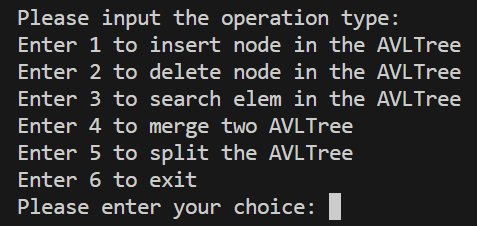
\includegraphics[width=13cm]{fig/AVLTree25.png}
  \caption{终端输入界面}
\end{figure}

上图为程序执行过程中用户看到的终端输入界面的提示,用户选择想要进行的操作并输入相应的数字即可继续下一步操作。

\begin{figure}[H]
  \centering
  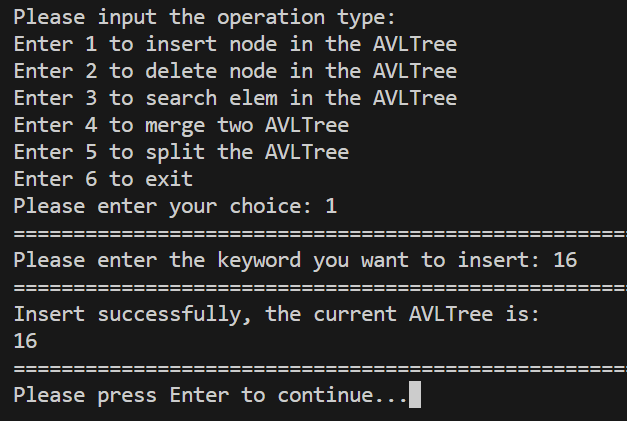
\includegraphics[width=13cm]{fig/AVLTree16.png}
  \caption{用户完成插入操作后的界面}
\end{figure}

提示用户输入需要插入的关键字后得出相应的平衡二叉树,然后用户需要按回车键继续下一步的操作。

我们提供了清屏功能,以保持当前界面始终保持整洁、美观,以免用户难以发现关键信息。

\begin{figure}[H]
  \centering
  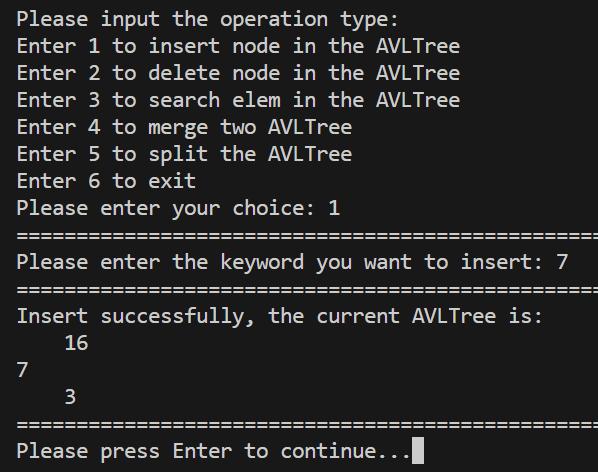
\includegraphics[width=13cm]{fig/AVLTree18.png}
  \caption{完成插入并平衡化之后的界面}
\end{figure}

如图所示,当我们依次插入16,3,7后,本应得到的二叉树是非平衡的,然后进行了平衡化处理,详细过程如下图所示:

\begin{figure}[H]
  \centering
  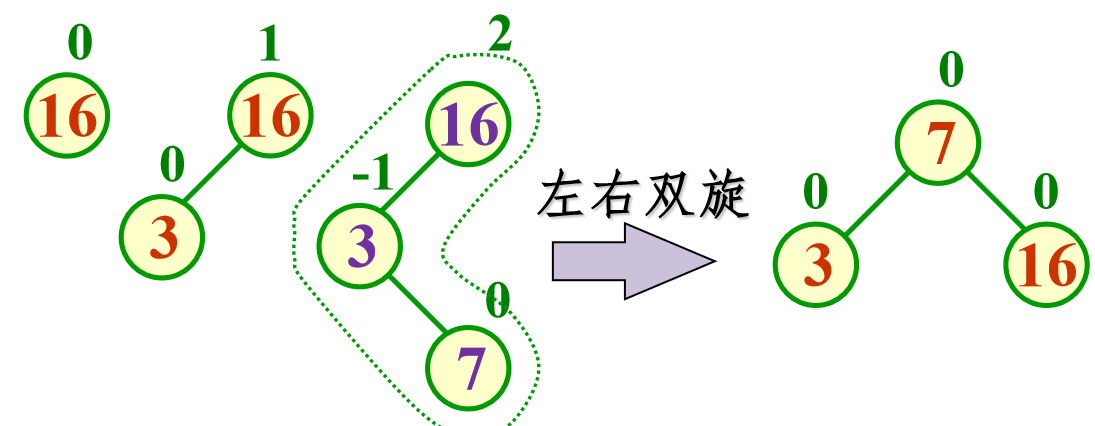
\includegraphics[width=13cm]{fig/AVLTree26.png}
  \caption{平衡化详细过程}
\end{figure}

然后依次插入11,9,26,18,14,15,最终得到的结果为:

\begin{figure}[H]
  \centering
  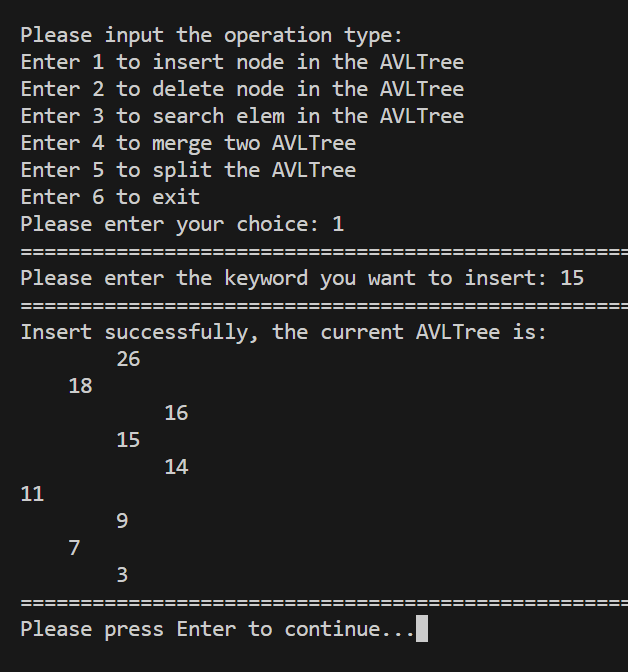
\includegraphics[width=13cm]{fig/AVLTree24.png}
  \caption{完成插入所有关键字后的界面}
\end{figure}

结果和PPT上例题中的结果一致。

注意到这里我们对于使用凹入表打印的优化,在OJ中的凹入表打印是如下图所示:

\begin{figure}[H]
  \centering
  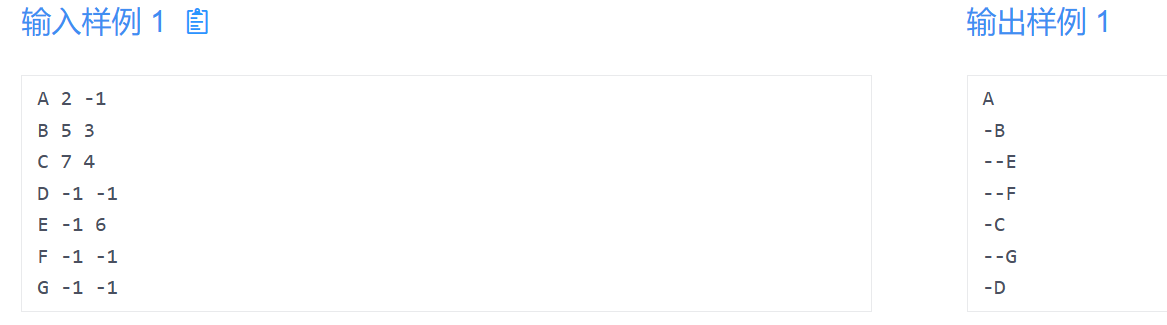
\includegraphics[width=13cm]{fig/AVLTree27.png}
  \caption{传统凹入表打印样式}
\end{figure}

虽然“-”的个数表示结点对应的层数,但是同一层的结点是分开的,不够直观的显示平衡二叉树的结构。

我们进行的优化是将树状图横置过来打印,即每一列表示平衡二叉树的每一层,结点右下方的结点为其左子节点,右上方的结点为其右子节点,能够直观的显示出平衡二叉树的特点。

关于删除结点,我们以删除叶子结点和根节点为例:

\begin{figure}[H]
  \centering
  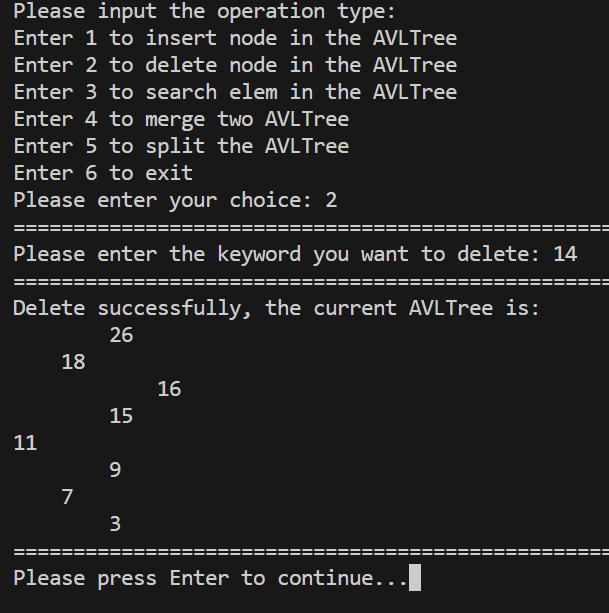
\includegraphics[width=13cm]{fig/AVLTree28.png}
  \caption{删除叶子结点后的界面}
\end{figure}

\begin{figure}[H]
  \centering
  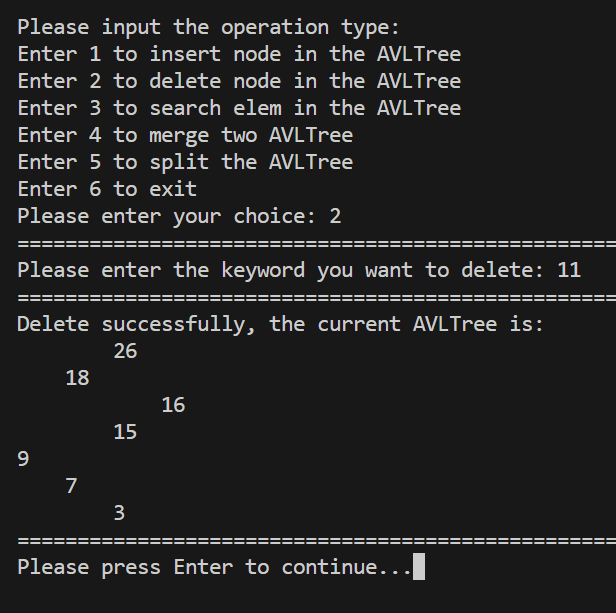
\includegraphics[width=13cm]{fig/AVLTree29.png}
  \caption{删除根结点后的界面}
\end{figure}

可以看出,删除叶子节点对于平衡没有影响,因此无需平衡化处理。

而删除根节点,则需要搜索其在中序次序下的直接前驱y,把结点y的内容传送给根节点,然后将问题转移到删除结点y,再进行平衡化处理。

对于查找操作的结果,则是若查找成功则输出查找成功,以及查找的关键字,若查找失败,则输出查找失败,关键字不存在的提示。

\vspace{1ex}

\noindent
$\bullet$
\textbf{合并、分裂操作的实例演示}。

合并操作要求我们输入两棵平衡二叉树的数据,并不一定要按照平衡二叉树的排序来输入,可以任意输入,然后程序会首先将其生成两棵平衡二叉树,再进行合并。

同时我们会将合并前的两棵平衡二叉树进行输出,以便用户观察和比较:

\begin{figure}[H]
  \centering
  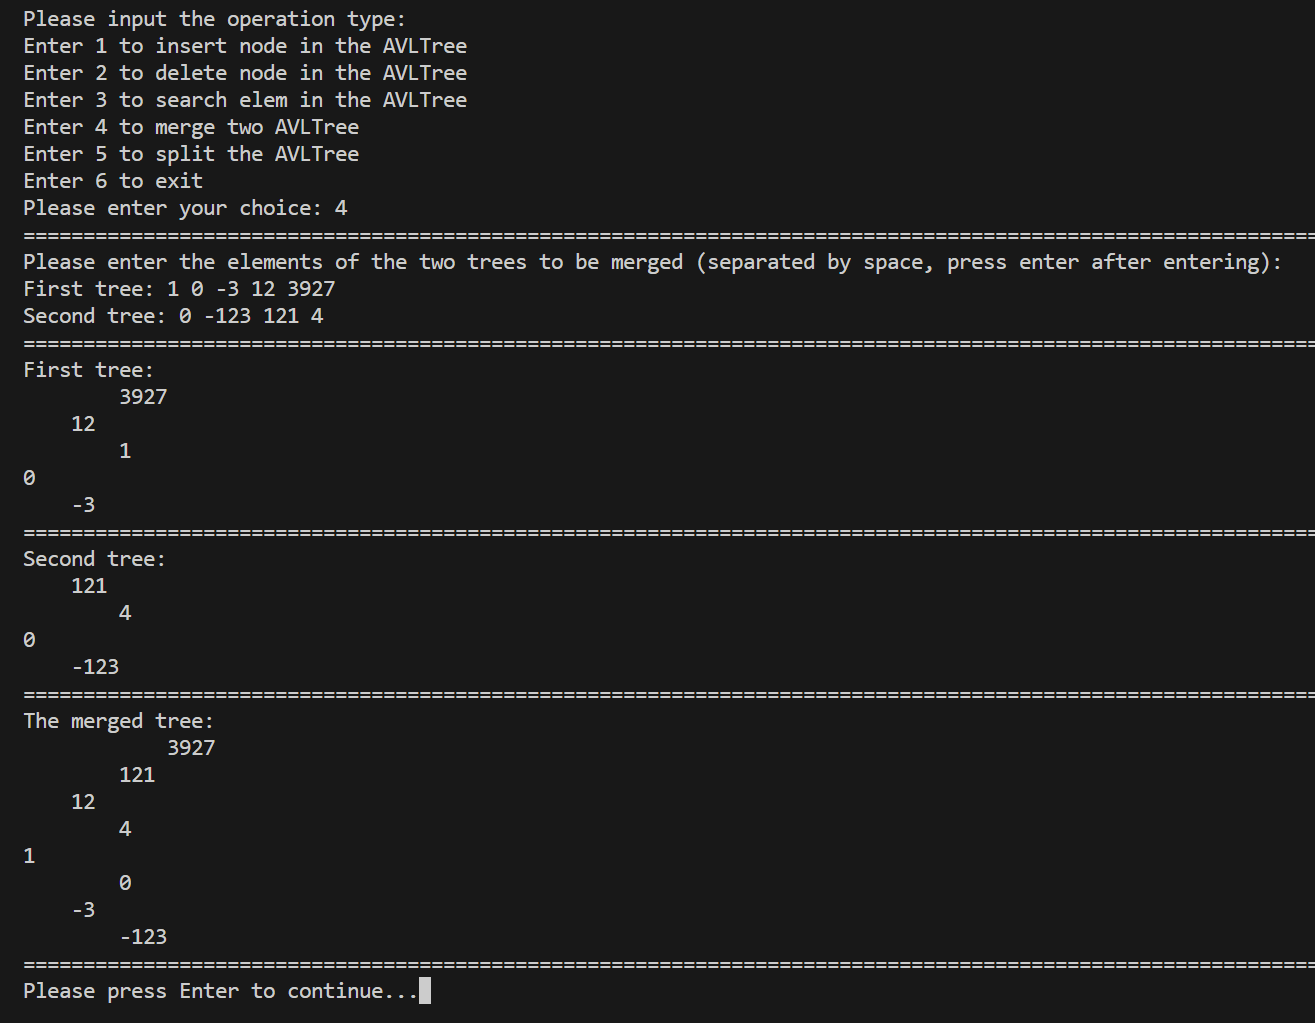
\includegraphics[width=15cm]{fig/AVLTree30.png}
  \caption{合并操作完成后的界面}
\end{figure}

上述合并操作的结果经验证为正确结果。

对于分裂操作,我们首先输入待分裂的平衡二叉树的数据,也不要求按照平衡二叉树的排序来输入,可以任意输入,然后程序会首先将其生成平衡二叉树,再输入分裂的标准关键字,然后程序根据标准关键字将该平衡二叉树分裂成满足要求的两棵平衡二叉树。

同样的,我们会输出分裂前和分裂后的平衡二叉树供用户观察和比较:

\begin{figure}[H]
  \centering
  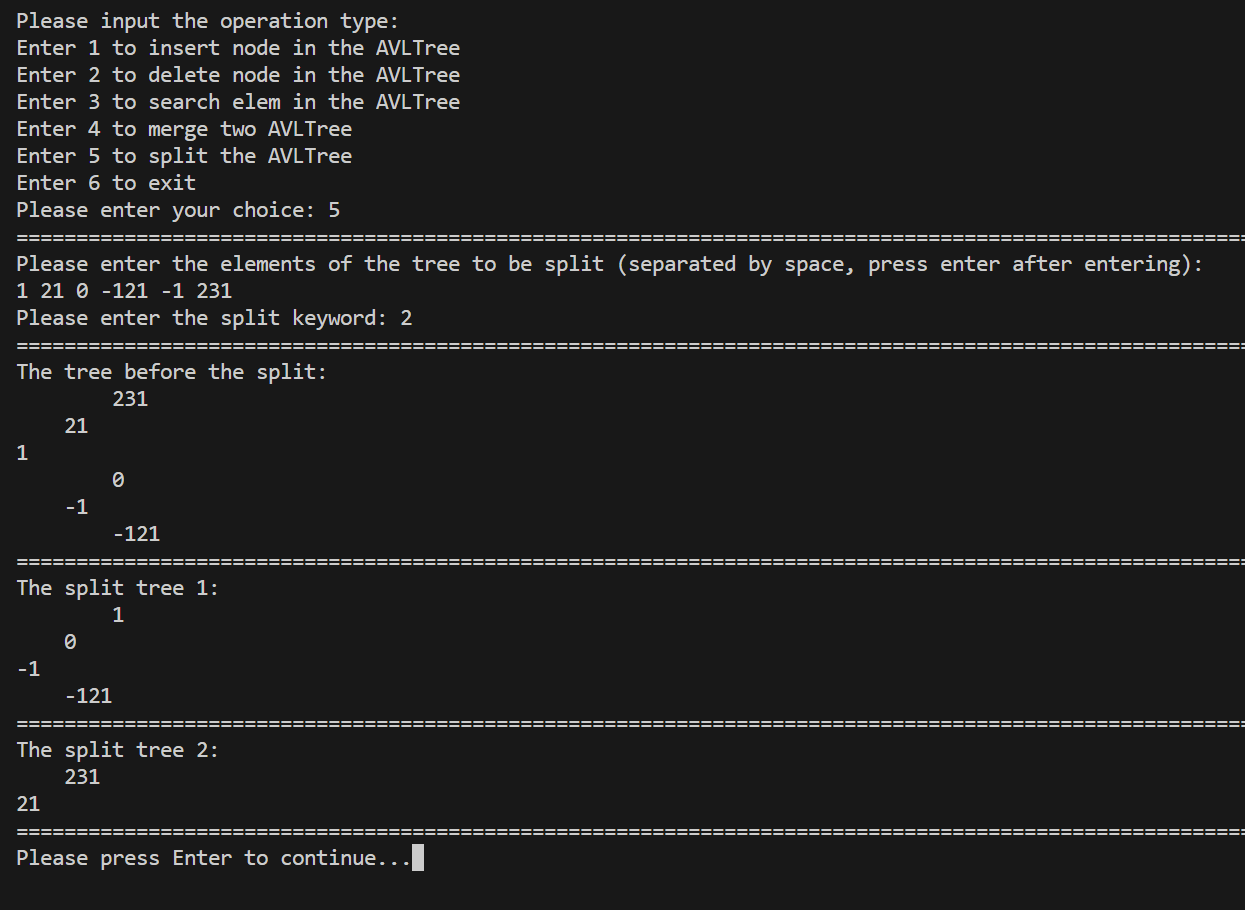
\includegraphics[width=15cm]{fig/AVLTree31.png}
  \caption{分裂操作完成后的界面}
\end{figure}

上述分裂操作的结果经验证也是正确的。

\vspace{1ex}

\noindent
$\bullet$
\textbf{优越性分析}

本实验中最大的优化就是降低了合并操作和分裂操作的时间复杂度。

按照原方法的合并操作,合并操作遍历树T2中的每个节点,并将其插入到T1中。T2中的每个节点插入到T1中的时间复杂度为O(log n1),其中n1是T1中的节点数。

因此,合并操作的时间复杂度为O(n2*log n1),其中n2是T2中的节点数。

合并操作的递归调用栈的深度为O(log n2),此外在插入结点时递归调用栈的深度为O(log n1),且需要额外增加O(n2)个结点。

因此,总空间复杂度为O(log n1 + log n2 + n2),即O(n)的空间复杂度。

而优化后的算法时间空间复杂度均为O(n1 + n2),在空间上二者相当,但是在时间上有较大的优化。

同样的,对于分裂操作,原方法分裂操作遍历树R中的每个节点,并将其插入到T1或T2中。R中的每个节点插入到T1或T2中的时间复杂度为 O(log n),其中n是T1或T2中的节点数。

因此,分裂操作的时间复杂度为O(n*log n),其中n是R中的节点数。

分裂操作的递归调用栈的深度为O(log n),此外在插入结点时需要额外增加O(n)个结点。

因此,总空间复杂度为O(n)。

而优化后的算法时间空间复杂度均为O(n1 + n2),在空间上二者相当,但是在时间上同样有较大的优化。
